\documentclass[nostrict]{szablonPG}

%-------------------- Dodatkowe pakiety ---------------------

%%\usepackage[utf8]{inputenc}
\usepackage{algorithm}
\usepackage{algorithmic}
%\usepackage{subcaption}
\usepackage{amsfonts} 
\usepackage{lmodern}
\usepackage{array}
\usepackage{mathtools}
\usepackage{tikz} 
\usepackage{graphicx}

%\usepackage{listing_schemat}
\usepackage[T1]{fontenc}
\usepackage[polish]{babel}

%------------------------------------------------------------
\usetikzlibrary{graphs,graphs.standard,quotes}
\selectlanguage{polish}
\newtheorem{theorem}{Twierdzenie} 
\newtheorem{definition}{Definicja}
\makeatletter
\renewcommand{\ALG@name}{Algorytm}
\makeatother
%------------------------------------------------------------
%			      Pocz�tek pracy dyplomowej  
%------------------------------------------------------------

\begin{document}

%------------------------------------------------------------
%  Dodanie strony tytu�owej wygenerowanej z MojaPG oraz 
%  						o�wiadczenia

%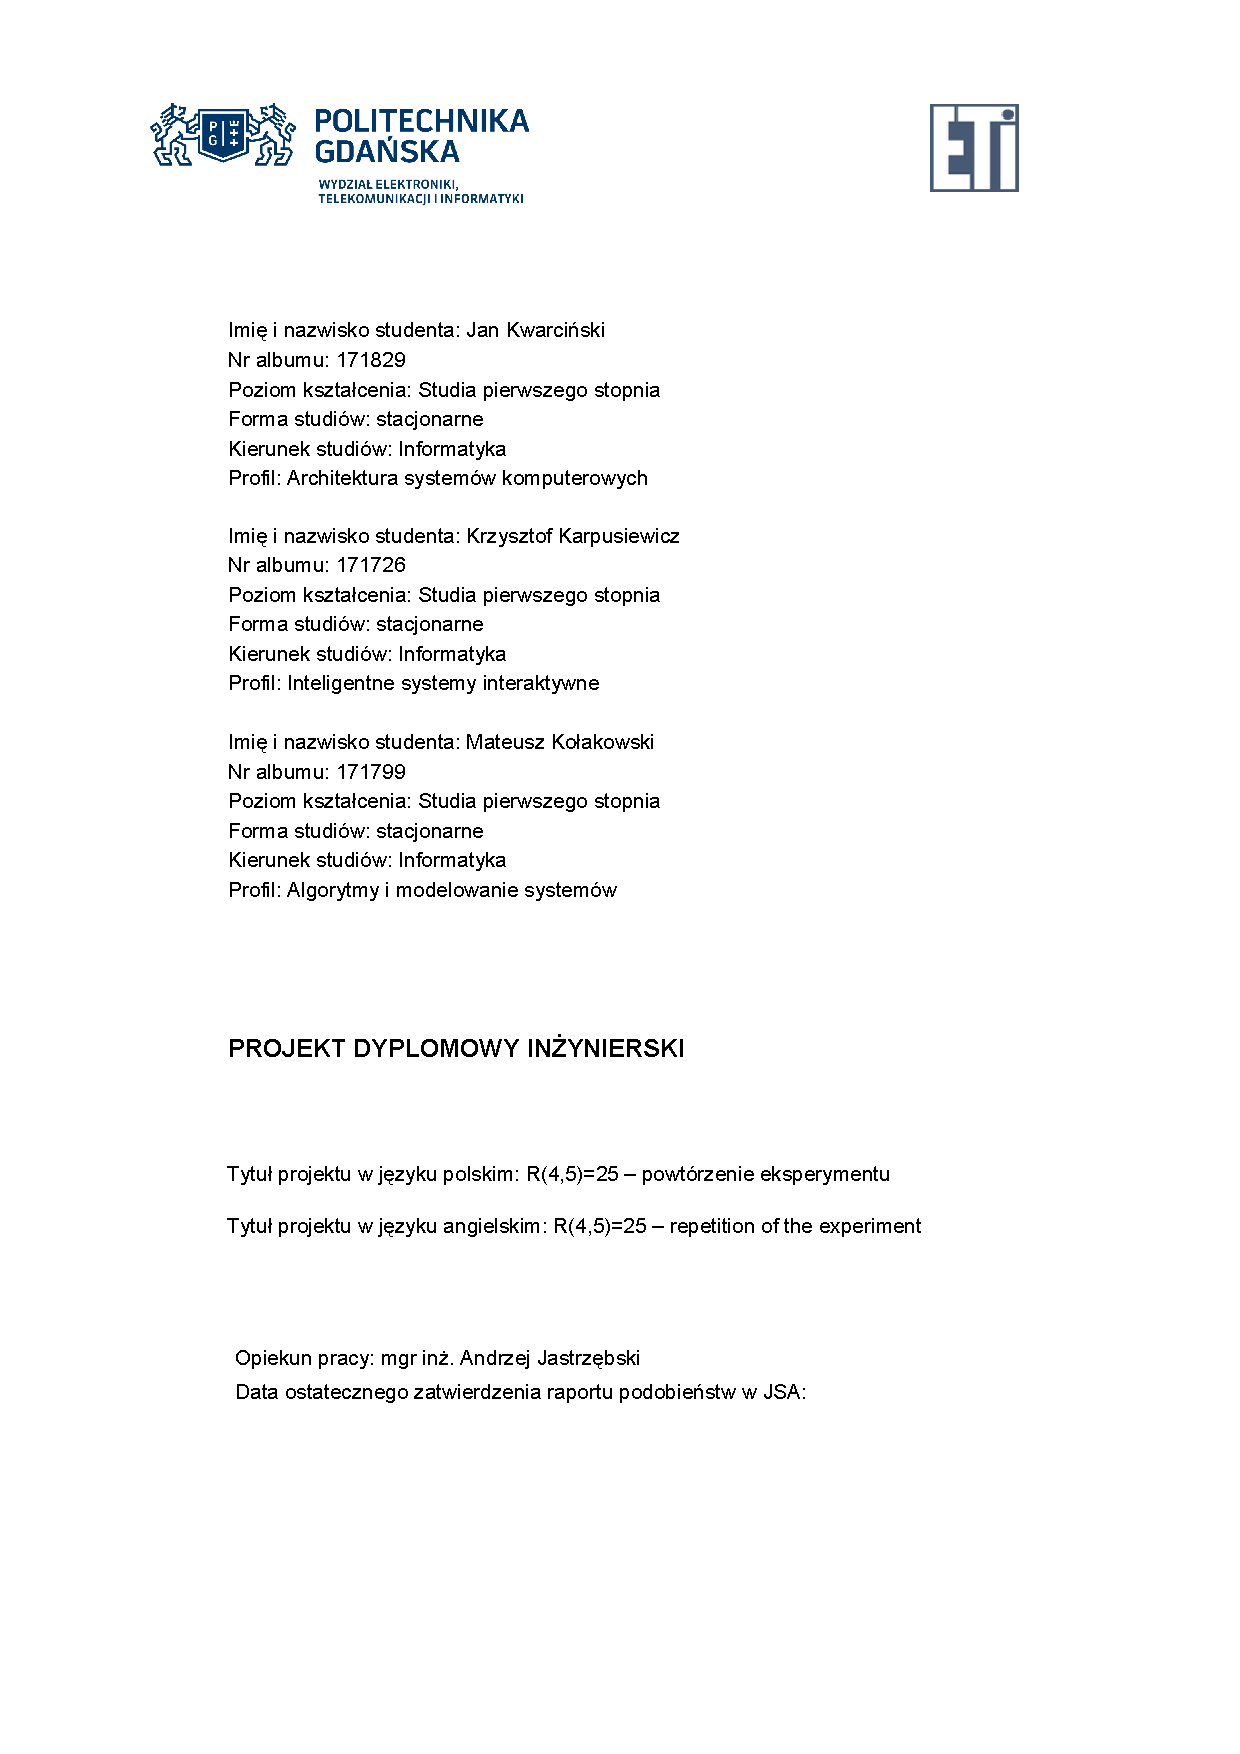
\includepdf{meta/strona_tytulowa.pdf}
%\includepdf{meta/oswiadczenie.pdf}

%------------------------------------------------------------
%  Dodanie streszczenia i abstract
%  						

%\chapter*{Streszczenie}
\indent Lorem Lorem ipsum dolor sit amet, consectetur adipiscing elit. Vivamus elementum arcu nec blandit aliquam. Integer eros dolor, molestie eget dictum quis, luctus sit amet sapien. Proin dignissim felis in ornare volutpat. Morbi vulputate rutrum efficitur. Ut vehicula vehicula metus, et iaculis tortor mattis vel. Nam blandit, arcu quis ultricies blandit, libero ante commodo augue, in accumsan dui leo at orci. Phasellus in augue et velit pulvinar malesuada ut et sem. Nulla vehicula nibh eu odio sollicitudin sagittis. Praesent condimentum semper neque, tincidunt luctus nisl scelerisque sed. Orci varius natoque penatibus et magnis dis parturient montes, nascetur ridiculus mus. 
\vspace{0.5cm}\newline
\textbf{S�owa kluczowe:} lorem ipsum, dolor sit amet, consectetur adipiscing\vspace{0.5cm}

\noindent \textbf{Dziedzina nauki i techniki, zgodnie z wymogami OECD:} nauki in�ynieryjne i techniczne, robotyka i automatyka

%\chapter*{Abstract}
\indent This paper describe.... Lorem ipsum dolor sit amet, consectetur adipiscing elit. Vivamus elementum arcu nec blandit aliquam. Integer eros dolor, molestie eget dictum quis, luctus sit amet sapien. Proin dignissim felis in ornare volutpat. Morbi vulputate rutrum efficitur. Ut vehicula vehicula metus, et iaculis tortor mattis vel. Nam blandit, arcu quis ultricies blandit, libero ante commodo augue, in accumsan dui leo at orci. Phasellus in augue et velit pulvinar malesuada ut et sem. Nulla vehicula nibh eu odio sollicitudin sagittis. Praesent condimentum semper neque, tincidunt luctus nisl scelerisque sed. Orci varius natoque penatibus et magnis dis parturient montes, nascetur ridiculus mus. 
\vspace{0.5cm}\newline
\textbf{Keywords:} lorem ipsum, dolor sit amet, consectetur adipiscin \vspace{0.5cm}

%------------------------------------------------------------
%	Utworzenie spisu tre�ci pracy dyplomowej
\tableofcontents

%------------------------------------------------------------
%	Dodanie wykazu wazniejszych skr�t�w i oznacze� 
%%\chapter*{Wykaz wa�niejszych oznacze� i skr�t�w} % section* - ukrywa numerowanie oraz wyklucza ze spisu tresci
\addcontentsline{toc}{chapter}{Wykaz wa�niejszych oznacze� i skr�t�w}% % reczne dodanie do spisu tresci
\noindent PWM -- Pulse Width Modulation\newline
ADC -- Analog-to-Digital Converter \newline
SPI -- Serial Pheripheral Interface\newline
PCB -- Printed Circuit Board\newline


%------------------------------------------------------------
%	Dodanie rozdzia��w pracy dyplomowej - g��wne cia�o dokumentu 

\chapter{Wstęp}

\textit{Autor rozdziału: Jan Kwarciński}
\vspace{0.5cm}\newline
Nasza praca opiera się na publikacji R(4,5) = 25 wydanej w 1995 przez Brendana D. McKaya oraz Stanisława P. Radziszowskiego  \cite{mainpaper}. Motywacją do sporządzenia pracy było udowodnienie, że dokładna wartość liczby Ramseya R(4,5) wynosi 25, z wykorzystaniem nowych technologii. Prace nad wyznaczeniem wartości R(4,5) zaczęły się w 1955 wraz z wydaniem przez Greenwooda oraz Gleasona\cite{gandg} artykułu w którym wyznaczyli oni górną granicę $R(4,5) \leq 31$. W kolejnych latach granica ta była zawężana aż do $25 \leq R(4,5) \leq 27$ \cite{jgbound, mrbound}.\par
Wygenerowanie wszystkich możliwych dwukolorowych grafów a następnie sprawdzenie ich poprawności byłoby zbyt czasochłonne, więc wymagane jest inne podejście do problemu. Wykorzystano jedynie wyselekcjonowane grafy ($s$,$t$,$n$) gdzie $s$ oznacza rozmiar maksymalnej kliki, która znajduje się w grafie, $t$ oznacza wielkość maksymalnego zbioru niezależnego, który należy do grafu, a $n$ oznacza liczbę wierzchołków na których zbudowany jest graf. Celem było skonstruowanie rodziny grafów R(4,5,24) z grafów R(3,5,d) oraz R(4,4,24-d) gdzie 7 $\leq$ d $\leq$ 13, z użyciem algorytmu ''sklejania''. Ostatnim krokiem przed weryfikacją wyników jest próba rozszerzenia otrzymanych grafów R(4,5,24) o jeden wierzchołek.

W naszej pracy omawiamy techniki i algorytmy służące do przeprowadzenia powyższego dowodu, oraz opisujemy dokonaną implementację.

Autorzy poszczególnych części:
\begin{itemize}
\item Podstawy teoretyczne: Mateusz Kołakowski
\item Twierdzenie Ramseya:  Jan Kwarciński
\item Generowanie grafów: Mateusz Kołakowski, Krzysztof Karpusiewicz
\item Rozszerzanie grafów: Krzysztof Karpusiewicz
\item Generowanie grafów nieizomorficznych: Mateusz Kołakowski
\item Generowanie grafów Ramseyowskich: Krzysztof Karpusiewicz, Mateusz Kołakowski
\item Sklejanie grafów: Mateusz Kołakowski, Jan Kwarciński, Krzysztof Karpusiewicz
\item Dekompozycja problemu: Mateusz Kołakowski
\item Grafy potrzebne do sklejania: Krzysztof Karpusiewicz
\item Algorytm sklejania: Krzysztof Karpusiewicz
\item Zawężanie przedziałów - zasady A-D: Mateusz Kołakowski, Jan Kwarciński
\item Rozszerzenie grafu R(4,5,24) do R(4,5,25): Krzysztof Karpusiewicz
\item Implementacja i eksperymenty: Mateusz Kołakowski, Jan Kwarciński, Krzysztof Karpusiewicz
\end{itemize}



\chapter{Podstawy teoretyczne} 
\textit{Autor rozdziału: Mateusz Kołakowski}
\vspace{0.5cm}\newline
Przed omówieniem tematu naszej pracy, należy przedstawić kilka pojęć z teorii grafów, bez których zrozumienia, nie jest możliwe wyznaczanie liczb Ramseya.

  \section{Teoria grafów}
  \begin{definition}[Graf prosty]
    Graf prosty G składa się z niepustego, skończonego zbioru wierzchołków $V(G)$, oraz skończonego zbioru krawędzi $E(G)$, który zawiera dwuelementowe podzbiory $\{u,v\} \in V(G)$. Dodatkowo, można powiedzieć, że dla każdego $\{u,v\} \in E(V) \Rightarrow u \neq v$ oraz $E(V)$ nie zawiera duplikatów. \cite{graphtheory}
  \end{definition}

  Dla potrzeb naszej pracy, będziemy zakładać, że gdy mówimy o grafie, mamy na myśli graf nieskierowany i prosty.
  
  \begin{definition}[Rząd grafu]
   Rząd grafu to liczba elementów zbioru $V$ w grafie $G=(V, E)$.
  \end{definition}

  Rząd grafu to liczba jego wierzchołków. 
  
       \begin{definition}[Podgraf indukowany]
       Dla grafu $G=(V,E)$ i podzbioru jego wierzchołków $S \subseteq V$, 
       podgrafem indukowanym $G[S]$ nazywamy taki graf, którego wszystkie wierzchołki
       zawierają się w $S$ i którego zbiór krawędzi zawiera wszystkie krawędzie z $E$ kończące się w $S$. 
       \begin{align*}
       G[S] = H(S, E_2) \textrm{ gdzie }  E_2=\{\{u,v\}:\{u,v\} \in E \wedge u,v \in S\}
       \end{align*}
     \end{definition}

     Na potrzeby naszej pracy mówiąc o podgrafie mamy na myśli podgraf indukowany.

  \begin{definition}[Sąsiedztwo]
    W grafie $G=(V, E)$ wierzchołki $u, v \in V$ sąsiadują wtedy i tylko wtedy gdy $\{u, v\} \in E$.    
  \end{definition}
  W grafach nieskierowanych sąsiedztwo jest relacją symetryczną. Jest nieprzechodnia - z sąsiedztwa $u$ i $v$ oraz $v$ i $w$ nie wynika sąsiedztwo $u$ i $w$ (Patrz rysunek \ref{sasie}).

  \begin{figure}[H]
    \centering
    \begin{tikzpicture}[node distance={15mm}, main/.style = {draw, circle}] 
      \node[main] (1) {$1$};
      \node[main] (2) [below right of=1] {$5$};
      \node[main] (3) [above right of=2] {$2$};
      \node[main] (4) [below left of=2] {$4$};
      \node[main] (5) [below right of=2] {$3$};

      \draw (1) -- (2);
      \draw (2) -- (3);
      \draw (2) -- (4);
      \draw (2) -- (5);
      \draw (1) -- (3);
      \draw (4) -- (5);
    \end{tikzpicture}
    \caption{Graf, w którym wierzchołek 1 sąsiaduje z 2 i 5; 2 z 1 i 5; 3 z 4 i 5; 4 z 3 i 5; 5 z 1, 2, 3 i 4 }
    \label{sasie}
  \end{figure}
  
     \begin{definition}[Stopień wierzchołka]
	Stopniem wierzchołka $v$ nazywamy ilość wierzchołków sąsiadujących z nim.
   \end{definition}
   
    \begin{definition}[Stopień grafu]
 Stopniem grafu nazywamy maksymalny stopień jego wierzchołków. 
   \end{definition}

   \begin{definition}[Klika]
    Klika $K$ w grafie $G=(V,E)$ jest takim podzbiorem wierzchołków $V(G)$, że dla każdej pary wierzchołków $u, v \in K$ zachodzi $$\{u,v\} \in E(G)$$ 
   \end{definition}
   
   W uproszczeniu, klika to podzbiór wierzchołków grafu, z których każdy jest połączony z każdym innym wiechołkiem tego podzbioru. Przykład grafu zawierającego klikę można zobaczyć na rysunku \ref{klik}
   \begin{figure}[H]
   \centering
    \begin{tikzpicture}[node distance={15mm}, main/.style = {draw, circle}] 
      \node[main] (1) {$1$};
      \node[main] (3) [below right of=1] {$3$};
      \node[main] (2) [below left of=3] {$2$};
      \node[main] (4) [below right of=3] {$4$};
      \node[main] (5) [above right of=3] {$5$};
      
      \draw (3) -- (2);
      \draw (1) -- (3);
      \draw (1) -- (2);
      \draw (2) -- (4);
      \draw (4) -- (5);
      \draw (1) -- (5);
     \end{tikzpicture}
     \caption{Wierzchołki 1, 2, 3 tworzą klikę stopnia 3 - $K_3$ }
     \label{klik}
  \end{figure}

  Znalezienie stopnia maksymalnej kliki w danym grafie jest trudne obliczeniowo.
  W ogólności jest to problem rozwiązywany w czasie niewielomianowym (chociaż dla niektórych grup grafów, 
  takich jak grafy planarne, istnieją algorytmy wielomianowe), ale sprawdzenie czy w grafie istnieje klika
  z góry znanego stopnia, jest wielomianowe. Przykładowo istnienie $K_3$ możemy sprawdzić następującym algorytmem:
  
  
  \begin{algorithm}
    \caption{Sprawdzenie czy graf zawiera $K_3$}
    \begin{algorithmic}
    \REQUIRE $G(V, E) $
    \FORALL{$v \in V$}
      \FORALL{$u \in V$}
        \IF{$v \neq u \land v \in$ sąsiedzi($u$) $\land$ sąsiedzi($v$) $\cap$ sąsiedzi($u$) $\neq \emptyset$}
          \STATE \RETURN jest $K_3$
        \ENDIF
      \ENDFOR
    \ENDFOR
    \STATE \RETURN nie ma $K_3$
    \end{algorithmic}
  \end{algorithm}
  
  
  \begin{definition}[Zbiór niezależny]
    Zbiór niezależny $N$ w grafie $G=(V,E)$ to taki podzbiór wierzchołków grafu $G$, że dla każdej pary wierzchołków $u, v \in N$ zachodzi $$\{u,v\} \notin E(V) $$. 
  \end{definition}

    \begin{figure}[H]
      \centering
       \begin{tikzpicture}[node distance={15mm}, main/.style = {draw, circle}] 
         \node[main] (1) {$1$};
         \node[main] (3) [below right of=1] {$3$};
         \node[main] (2) [below left of=3] {$2$};
         \node[main] (4) [below right of=3] {$4$};
         \node[main] (5) [above right of=3] {$5$};

         \draw (2) -- (4);
         \draw (4) -- (5);

        \end{tikzpicture}
        \caption{Wierzchołki 1, 2, 3, 5 tworzą zbiór niezależny 4 - $N_4$ }
        \label{zniez}
     \end{figure}


     Zbiór niezależny można również zdefiniować jako przeciwieństwo kliki, lub jako klikę w dopełnieniu grafu. Rysunek \ref{zniez} prezentuje przykład zbioru niezależnego.

    \begin{definition}[Dopełnienie grafu]
      Depełnieniem grafu $G=(V,E)$ nazywamy taki graf $G'=(V,E')$, 
      dla którego zachodzi 
      $$\forall_{u,v} \{u,v\} \in E \iff \{u,v\} \notin E'$$
    \end{definition}
  
     Natychmiast zauważamy, że graf $G'$ posiada klikę $K_3$:
    Oznacza to, że $G$ ma $N_3$ na tych samych wierzchołkach (rysunek \ref{dopwiesz}).

    \begin{figure}[H]
      \centering
\subfloat[]{
       \begin{tikzpicture}[node distance={15mm}, main/.style = {draw, circle}] 
        \node[main] (1) at (0:2){$1$};
        \node[main] (3) at (72:2) {$3$};
        \node[main] (2) at (144:2) {$2$};
        \node[main] (4) at (216:2) {$4$};
        \node[main] (5) at (288:2) {$5$};

         \draw (1) -- (3);
         \draw (2) -- (4);
         \draw (3) -- (5);
         \draw (3) -- (4);
         \draw (4) -- (5);

         \draw[red, dashed] (1) -- (2);
         \draw[red, dashed] (1) -- (5);
         \draw[red, dashed] (2) -- (5);

        \end{tikzpicture}
}
        \hspace{15mm}
 \subfloat[]{
       \begin{tikzpicture}[node distance={15mm}, main/.style = {draw, circle}] 
         \node[main] (1) at (0:2){$1$};
         \node[main] (3) at (72:2) {$3$};
         \node[main] (2) at (144:2) {$2$};
         \node[main] (4) at (216:2) {$4$};
         \node[main] (5) at (288:2) {$5$};

         \draw[red] (1) -- (2);
         \draw[red] (1) -- (5);
         \draw (2) -- (3);
         \draw[red] (2) -- (5);

        \end{tikzpicture}
}
        \caption{ $K_3$ w $G'$ leży między tymi samymi Wierzchołkami co $N_3$ w $G$ }
        \label{dopwiesz}
     \end{figure}




  \section{Izomorfizm}

  \begin{definition}[Izomorfizm grafów]
    Izomorfizm grafów $G$ i $H$ to taka biekcja $f:V(G) \to V(H)$, że 2 wierzchołki $u$ i $v$ sąsiadują w $G$ wtedy i tylko wtedy gdy $f(u)$ i $f(v)$ sąsiadują w $H$.
  \end{definition}

  Innymi słowy, izomorfizm jest to takie przekształcenie grafu, które zachowuje wszystkie jego właściwości. Grafy, dla których można znaleźć izomorfizm są izomorficzne\cite{graphtheory}. Czyli, dwa grafy są izomorficzne, jeżeli ich wierzchołki można nazwać w taki sposób, 
  aby odpowiadające sobie wierzchołki w obu grafach miały dokładnie takie same zbiory sąsiadów.
  

  Przekształćmy graf z rysunku \ref{sasie} zamieniając wierzchołek 1 z 2 oraz 3 z 4:
  \begin{figure}[H]
    \centering
    \subfloat[]{
 \begin{tikzpicture}[node distance={15mm}, main/.style = {draw, circle}] 
      \node[main] (1) {$1$};
      \node[main] (2) [below right of=1] {$5$};
      \node[main] (3) [above right of=2] {$2$};
      \node[main] (4) [below left of=2] {$4$};
      \node[main] (5) [below right of=2] {$3$};

      \draw (1) -- (2);
      \draw (2) -- (3);
      \draw (2) -- (4);
      \draw (2) -- (5);
      \draw (1) -- (3);
      \draw (4) -- (5);
    \end{tikzpicture}
    }
    \hspace{15mm}
    \subfloat[]{
    \begin{tikzpicture}[node distance={15mm}, main/.style = {draw, circle}] 
      \node[main] (1) {$2$};
      \node[main] (2) [below right of=1] {$5$};
      \node[main] (3) [above right of=2] {$1$};
      \node[main] (4) [below left of=2] {$3$};
      \node[main] (5) [below right of=2] {$4$};

      \draw (1) -- (2);
      \draw (2) -- (3);
      \draw (2) -- (4);
      \draw (2) -- (5);
      \draw (1) -- (3);
      \draw (4) -- (5);
    \end{tikzpicture}
    }
    \caption{Mimo przekształcenia graf zachował swoje własności}
    \label{sasieizo}
  \end{figure}

  Jak widać na rysunku \ref{sasieizo}, wierzchołki o tych samych numerach zachowały swoje zbiory sąsiadów. 

  Wszystkie własności opisane w tej pracy są przez izomorfizmy niezmienione, a więc na nasz użytek dwa grafy izomorficzne to efektywnie ten sam graf.


  \begin{definition}[Automorfizm grafu]
    Automorfizm grafu $G$ to taka permutacja $f$ zbioru wierzchołków $G$, że para wierzchołków $u$, $v$ jest sąsiedująca tylko jeżeli $f(u)$ i $f(v)$ sąsiadują\cite{graphtheory}.
  \end{definition}
  Automorfizm to izomorfizm z grafu początkowego do tego samego grafu. 
  Złożenie automorfizmów również jest automorfizmem.  

  \begin{definition}[Grupa automorfizmu]
    Grupa automorfizmów grafu $G$ to zbiór składający się z wszystkich automorfizmów grafu $G$.
  \end{definition}

  \section{Formy kanoniczne grafów}

  \begin{definition}[Forma kanoniczna]
    Forma kanoniczna $C(G)$ grafu $G$ to taki graf izomorficzny do $G$, że każdy graf izomorficzny do $G$ ma taką samą formę kanoniczną\cite{canon}. 
    $$ Canon \colon G \to F$$
    $$G \simeq H \iff Canon(G) = Canon(H) $$
  \end{definition}

  Forma kanoniczna grafu to takie przekształcenie $G$, 
  które daje identyczny wynik dla wszystkich grafów izomorficznych z $G$. Przykładowo, takie przekształcenie można zaimplementować
   jako numerowanie wierzchołków począwszy od takich o najmniejszej liczbie sąsiadów. 
   %Jeżeli kilka wierzchołków ma taką samą liczbę sąsiadów to albo niższy numer otrzymuje 		wierzchołek, 
   %który ma sąsiada (sąsiadów) z najniższym numerem albo losowy. NIE DO KOŃCA PRAWIDLOWE


%   \begin{algorithm}[H]
%    \caption{Sprowadzenie grafu do formy kanonicznej}
%    \begin{algorithmic}
%    \REQUIRE $G(V, E) $
%    \STATE tab = sort($V$, iloscSasiadowRekurencyjnie)
%    \FORALL{$v \in V(G)$}
%      \STATE $v.numer = tab.indeks(v) $
%    \ENDFOR
%    \end{algorithmic}
%  \end{algorithm}
  
%  Powyższy algorytm poprawnie tworzy formy kanoniczne jedynie dla bardzo prostych grafów.
%  Rzeczywiste algorytmy są dużo bardziej zoptymalizowane i Korzystają z 
%  heurystyk pozwalających zoptymalizować proces dla określonych przypadków\cite{canon}.
%  Sprowadzanie do formy kanonicznej jest kluczowe dla szybkiego wyszukiwania izomorfizmów.
Algorytmy tworzące formy kanoniczne korzystają z  heurystyk pozwalających zoptymalizować proces dla określonych przypadków\cite{canon}.  Sprowadzanie do formy kanonicznej jest kluczowe dla szybkiego wyszukiwania izomorfizmów.
%
 

\begin{definition}[Orbita]
  Orbita w grafie $G$ to taki maksymalny zbiór będący podzbiorem zbioru wierzchołków, taki dla każdych dwóch elementów tego zbioru da się znaleźć automorfizm przekształcający jeden element w drugi.
\end{definition}

Wszystkie wierzchołki wewnątrz orbity mogą zostać dowolnie zamienione, nie zmieniając właściwości grafu. Ich zamiana jest automorfizmem.
Przykład (rysunek \ref{orbit}): 
\begin{figure}[H]
  \centering
   \begin{tikzpicture}[node distance={15mm}, main/.style = {draw, circle}] 
     \node[main] (1) {$1$};  
     \node[main] (3) [right of=1] {$3$};
     \node[main] (2) [above of=3] {$2$};
     \node[main] (4) [below of=3] {$4$};
     \node[main] (5) [right of=3] {$5$};

     \draw (1) -- (3);
     \draw (1) -- (2);
     \draw (1) -- (4);
     \draw (5) -- (2);
     \draw (5) -- (3);
     \draw (5) -- (4);
    \end{tikzpicture}
    \caption{Orbita pierwsza: 1, 5; Orbita druga: 2, 3, 4}
    \label{orbit}
 \end{figure}


    \section{Kolorowanie grafu}
    \begin{definition}[Oznakowanie grafu]
      Dla grafu $G=(V, E)$, wierzchołkowym oznakowaniem grafu nazywamy funkcję
       mapującą wierzchołki do oznaczeń (rysunek \ref{kolor1}). Analogicznie, funkcję mapującą krawędzie do oznaczeń 
       nazywamy krawędziowym oznakowaniem grafu (rysunek \ref{kolor2}).  
    \end{definition}


    \begin{figure}[H]
      \centering
       \begin{tikzpicture}[node distance={30mm}, main/.style = {draw, circle}] 
         \node[main] (1) {Gdańsk};
         \node[main] (3) [below right of=1] {Warszawa};
         \node[main] (2) [below left of=3] {Olszyn};
         \node[main] (4) [below right of=3] {Kraków};
         \node[main] (5) [above right of=3] {Rzeszów};

         \draw (2) -- (4);
         \draw (4) -- (5);

        \end{tikzpicture}
        \caption{ Przykład wierzchołkowego oznakowania grafu $G$ z rysunku }
        \label{kolor1}
     \end{figure}

     \begin{figure}[H]
      \centering
       \begin{tikzpicture}[node distance={30mm}, main/.style = {draw, circle}] 
         \node[main] (1) {$1$};
         \node[main] (3) [below right of=1] {$3$};
         \node[main] (2) [below left of=3] {$2$};
         \node[main] (4) [below right of=3] {$4$};
         \node[main] (5) [above right of=3] {$5$};

         \draw (2) -- (4) node [midway, fill=white] {autostrada};
         \draw (4) -- (5) node [midway, fill=white] {droga ekspresowa};

        \end{tikzpicture}
        \caption{ Przykład krawędziowego oznakowania grafu $G$ }
        \label{kolor2}
     \end{figure}

     Oznakowywanie elementów grafów ma wiele zastosowań. Często nadaje się krawędziom wartości mające reprezentować np.
     koszt pokonania drogi między dwoma punktami. Innym często wykorzystywanym oznakowaniem grafów jest kolorowanie.   
   
    \begin{definition}[Kolorowanie grafu]
      Kolorowanie grafów jest szczególnym przypadkiem oznakowywania grafu w którym oznaczenia są nazywane kolorami i mogą być przypisywane tylko zgodnie z określonymi o
       ograniczeniami (rysunek \ref{kolor3} i \ref{kolor4}). 
    \end{definition}

    \begin{figure}[H]
      \centering
       \begin{tikzpicture}[node distance={15mm}, main/.style = {draw, circle}] 
     \node[main][red] (3) at (0:2) {$3$};
     \node[main][blue] (2) at (90:2) {$2$};
     \node[main][red] (1) at (180:2) {$1$};
     \node[main][blue] (4) at (270:2) {$4$};
    
    \draw[ultra thick] (4) -- (1);
    \draw[ultra thick] (3) -- (2);
    \draw[ultra thick] (1) -- (3);

    \draw[ultra thick] (2) -- (1);
    \draw[ultra thick] (2) -- (4);
    \draw[ultra thick] (1) -- (3);
        \end{tikzpicture}
        \caption{Przykładowe kolorowanie wierzchołkowe grafu}
        \label{kolor3}
     \end{figure}

    \begin{figure}[H]
      \centering
       \begin{tikzpicture}[node distance={15mm}, main/.style = {draw, circle}] 
     \node[main] (3) at (0:2) {$3$};
     \node[main] (2) at (90:2) {$2$};
     \node[main] (1) at (180:2) {$1$};
     \node[main] (4) at (270:2) {$4$};
    
    \draw[ultra thick][red] (4) -- (1);
    \draw[ultra thick][red] (3) -- (2);
    \draw[ultra thick][red] (1) -- (3);
    
    
    \draw[ultra thick][blue] (2) -- (1);
    \draw[ultra thick][blue] (2) -- (4);
    \draw[ultra thick][blue] (1) -- (3);
        \end{tikzpicture}
        \caption{Przykładowe kolorowanie krawędziowe grafu}
        \label{kolor4}
     \end{figure}

     Kolorowanie najczęściej idzie w parze z ograniczeniami, których należy przestrzegać przypisując elementom wartości.
     Najczęściej dotyczą one zakazu kolorowania sąsiadujących wierzchołków lub krawędzi tym samym kolorem. 
	
%     Innym ograniczeniem dla kolorowania może być zakaz pomalowania kliki ustalonego stopnia %$n$ - $K_n$ - tym samym kolorem.
%     Dla $n=2$ otrzymamy zakaz sąsiedztwa wspomniany wcześniej.
\chapter{Twierdzenie Ramseya}
Twierdzenie Ramseya mówi o konieczności pojawienia się pewnych układów w pozornym chaosie, co oznacza że każda większa struktura będzie zawierała jakąś podstrukturę. Zagadnienie można łatwo przedstawić posługując się teorią grafów, dla uproszczenia zostanie użyte kolorowanie dwoma kolorami.

\begin{theorem}
Niech $r \in \mathbb{N}$. Istnieje takie $n \in \mathbb{N}$  gdzie dla każdego 2-kolorowego $\mathit{K}_{n}$ grafu znajdzie się jednokolorowy podgraf $\mathit{K}_{r}$ w $\mathit{K}_{n}$.  \cite{theory} 
\end{theorem}

Z powyższego twierdzenia wynika, że będziemy omawiać dwukolorowe struktury. 

\begin{definition}[Liczba Ramseya]
Niech $r \in \mathbb{N}$ i $b \in \mathbb{N}$. Liczba Ramseya, wyrażana jako $n = R(r,b)$, jest najmniejszą liczbą całkowitą taką że 2-kolorowy graf $\mathit{K}_{n}$, używając koloru czerwonego i niebieskiego do kolorowania krawędzi, implikuje czerwony monochromatyczny podgraf $\mathit{K}_{r}$ lub niebieski monochromatyczny podgraf $\mathit{K}_{b}$
  \cite{theory} 
\end{definition}


W celu ułatwienia obliczeń i umożliwienia użycia technik generacji grafów, używamy uproszczenia reprezentacji grafowej. Zamiast wyznaczać kolorowania grafu pełnego, używamy wszystkich grafów prostych gdzie kolor krawędzi zamieniony jest na istnienie lub brak istnienia krawędzi pomiędzy parą wierzchołków.


\begin{definition}[Graf Ramseyowski]
Niech $r \in \mathbb{N}$, $b \in \mathbb{N}$ i $n \in \mathbb{N}$. Graf Ramseyowski, zapisany jako $R(r,b,n)$ oznacza graf mający $n$ wierzchołków, nie zawierający kliki o rozmiarze $r$ i nie zawierający zbioru niezależnego rozmiaru $b$.  \cite{theory} 
\label{gram}
\end{definition}

W kontekście tej pracy, określamy graf jako ramseyowski jeżeli nie posiada on kolorowania określonego w definicji \ref{gram}. Oznacza to, że graf spełniający R(4,5,6) to graf zbudowany na 6 wierzchołkach, który nie posiada kliki 4 rzędu ani zbioru niezależnego 5 rzędu. Przykładowy graf R(4,5,6) jest przedstawiony na rysunku \ref{pgram}

 \begin{figure}[H]
  \centering
   \begin{tikzpicture}[node distance={15mm}, main/.style = {draw, circle}] 
 \node[main] (3) at (0:2) {$3$};
 \node[main] (2) at (60:2) {$2$};
 \node[main] (1) at (120:2) {$1$};
 \node[main] (6) at (180:2) {$6$};
 \node[main] (5) at (240:2) {$5$};
 \node[main] (4) at (300:2) {$4$};

\draw[ultra thick] (6) -- (1);
\draw[ultra thick] (6) -- (2);
\draw[ultra thick] (6) -- (3);
\draw[ultra thick] (6) -- (4);
\draw[ultra thick] (6) -- (5);
\draw[ultra thick] (3) -- (4);
\draw[ultra thick] (2) -- (1);
    \end{tikzpicture}
    \caption{}
    \label{pgram}
 \end{figure}

Celem tej pracy jest wykazanie, że stworzenie grafu $R(4,5,25)$ jest niemożliwe, a istnieją grafy $R(4,5,24)$, z czego wynika, że liczba Ramseya $R(4,5) = 25$.


\section{Historia liczby i twierdzenia Ramseya}

W 1930 roku zostało opublikowane działo Franka Plumptona Ramseya ''On a Problem of Formal Logic''\cite{ramsey} , które posłużyło jako podstawę do teorii którą dzisiaj znamy jak Teoria Ramseya. 


\subsection{Twierdzenie Van der Waerden's}
Twierdzenie opublikowane przez Van der Waerdena w 1927 roku, przed powstaniem Twierdzenia Ramseya lecz uważana za jedną z jego gałęzi. 

\begin{theorem}
Dla dowolnych liczb naturalnych $r$ oraz $k$ istnieje taka liczba naturalna $n$ która określa zbiór \{1, 2, 3, ..., $n$\} który jest pokolorowany na $r$ różnych kolorów, z przynajmniej $k$ liczbami naturalnymi w ciągu arytmetycznym które są tego samego koloru.\cite{theory} 
\end{theorem}

Dla przykładu, $W(2,3) = 9$. Zbiór o ośmiu elementach można podzielić na następujące podzbiory aby w żadnym z podzbiorów nie wystąpił szereg arytmetyczny o trzech elementach, \{1,2,3,4,5,6,7,8\} $\to$ \{1,2,5,6\},\{3,4,7,8\}. W przypadku zbioru o dziewięciu elementach taki podział nie jest możliwy. Dodając 9 do dowolnego podzbioru utworzony zostanie ciąg arytmetyczny o trzech elementach np. \{1,5,9\} lub \{7,8,9\}. Podobna sytuacja zajdzie dla podziału \{1,4,5,8\},\{2,3,6,7\}

\subsection{Paul Erd\"os i teoria Ramseya}

Happy Ending problem, czyli problem zaprezentowany przez Paula Erd\"osa w 1933 roku brzmi następująco. 

\begin{theorem}
Dowolny zbiór 5 punktów w przestrzeni, w pozycja ogólna, zawiera podzbiór 4 punktów które formują wielokąt wypukły.
\end{theorem}

Twierdzenie to zostało uogólnione w 1935 roku przez George Szekeresa oraz Paula Erd\"osa

\begin{theorem}
Dla dowolnej liczby całkowitej N, każdy dowolnie duży i skończony zbiór punktów w przestrzeni, w pozycji ogólnej, zawiera podzbiór składający się z N punktów który tworzy wielokąt wypukły. \cite{erdoshappy} 
\end{theorem}

Prace nad Happy Ending problem sprawiły że Paul Erd\"os natrafił na publikacje Ramseya z 1928 roku. Spowodowało to że Erd\"os rozpoczął prace nad liczbami Ramseya, co przyczyniło się do rozwoju tej teorii.


\hfill  \par
Party problem lub inaczej Theorem on Friends and Strangers, jest to problem dzięki któremu można przedstawić przykład zastosowania liczby Ramseya. Brzmi on następująco: jaka jest najmniejsza liczba osób jaką trzeba zaprosić na przyjęcie tak aby trójka z nich były wspólnymi znajomymi lub trójka z nich była dla siebie nieznajomymi\cite{partyproblem}? Aby odpowiedzieć na to pytanie można zasięgnąć o pomoc do teorii Ramseya gdzie znajdziemy że odpowiedź na postawione pytanie stanowi liczba Ramseya $R(3,3)=6$ która jest opisana w dalszej części pracy. Powyższe pytanie można przedstawić w bardziej formalny sposób: Znajdź najmniejszą liczbę gości którzy muszą zostać zaproszeni tak aby przynajmniej $m$ znało się wzajemnie a $n$ była dla siebie obca \cite{partyformal}, lub inaczej; Znajdź najmniejszą liczbę wierzchołków dla których graf będzie zawierać klikę stopnia $n$ o kolorze czerwonym lub klikę stopnia $m$ o kolorze niebieskim. Rozwiązaniem dla tego problemu są liczby Ramseya. 


\section{Wartości liczb Ramseya}

\begin{enumerate}  

  \item $R(1,k)$ = $R(k,1)$ = 1 \hfill \par
  W przypadku gdy jeden z parametrów wynosi 1 aby spełnić warunek wystarczy jeden wierzchołek.  Jednokolorowy graf $\mathit{K}_{1}$ jest pojedynczym wierzchołkiem i spełnia zarówno warunek dla $R(1,b)$ oraz $R(r,1)$, patrz rysunek \ref{grafk1}. 
  
  \begin{figure}[h]
  \centering
  \begin{tikzpicture}[node distance={15mm}, main/.style = {draw, circle}] 
    \node[main] (1)  {$1$};

   \end{tikzpicture}
   \caption{R(1,k,1)}
   \label{grafk1}
\end{figure}
  
   \item $R(2,k)$ = $R(k,2)$ = $k$ \hfill \par
	W przypadku gdy jeden z parametrów wynosi 2 nie możemy postąpić analogicznie jak w przypadku gdy $k$=1, gdyż graf $\mathit{K}_{2}$ nie spełni warunku gdy $k$ > 2 dla kolorowania jednym kolorem. Tak samo każdy graf pełny o rozmiarze mniejszym niż $k$ nie spełnia warunku w sytuacji gdy zostanie użyty kolor ograniczony liczbą $k$ aby pokolorować go w jednolity sposób. Dlatego też liczba wierzchołków w grafie musi wynosić k co zawsze spełni jeden z dwóch warunków, pierwszy w przypadeu, gdy wszystkie krawędzie zostaną pokolorowane jednym kolorem lub drugi, gdy chociaż jedna krawędź będzie drugiego koloru. Przykładowo dla $R(2,4)$ gdzie pierwszy kolor (dla $r$=2) będzie oznaczony kolorem czerwonym a drugi ($b$=4) niebieskim, patrz rysunek \ref{grafk2}.
	
\begin{figure}[H]
  \centering
   \begin{tikzpicture}[node distance={15mm}, main/.style = {draw, circle}] 
 \node[main] (1) at (0:2) {$1$};
 \node[main] (2) at (90:2) {$2$};
 \node[main] (3) at (180:2) {$3$};
 \node[main] (4) at (270:2) {$4$};


\draw[ultra thick][blue] (1) -- (2);
\draw[ultra thick][blue] (1) -- (3);
\draw[ultra thick][blue] (1) -- (4);
\draw[ultra thick][blue] (2) -- (3);
\draw[ultra thick][blue] (2) -- (4);
\draw[ultra thick][red] (3) -- (4);

    \end{tikzpicture}
        \hspace{15mm}
       \begin{tikzpicture}[node distance={15mm}, main/.style = {draw, circle}] 
 \node[main] (1) at (0:2) {$1$};
 \node[main] (2) at (90:2) {$2$};
 \node[main] (3) at (180:2) {$3$};
 \node[main] (4) at (270:2) {$4$};


\draw[ultra thick][blue] (1) -- (2);
\draw[ultra thick][blue] (1) -- (3);
\draw[ultra thick][blue] (1) -- (4);
\draw[ultra thick][blue] (2) -- (3);
\draw[ultra thick][blue] (2) -- (4);
\draw[ultra thick][blue] (3) -- (4);
    \end{tikzpicture}
    \caption{Przykłady grafów niespełniających $R(2,4,4)$}
    \label{grafk2}
 \end{figure}
  	


  
 
  \item R(3,3)=6 \hfill \par
  R(3,3) jest pierwszym nietrywialnym przykładem liczby Ramseya, lecz nadal na tyle prostym aby łatwo móc ją wyznaczyć. Łatwo można wykluczyć $\mathit{K}_{3}$, $\mathit{K}_{4}$ oraz $\mathit{K}_{5}$ za pomocą następującego pokolorowania krawędzi (rysunek \ref{grafk5}).


\begin{figure}[H]
  \centering
   \begin{tikzpicture}[node distance={15mm}, main/.style = {draw, circle}] 
 \node[main] (1) at (1*90:2) {$1$};
 \node[main] (5) at (1*162:2) {$5$};
 \node[main] (4) at (1*234:2) {$4$};
 \node[main] (3) at (1*306:2) {$3$};
 \node[main] (2) at (1*18:2) {$2$};

\draw[ultra thick][red] (1) -- (2);
\draw[ultra thick][red] (2) -- (3);
\draw[ultra thick][red] (3) -- (4);
\draw[ultra thick][red] (4) -- (5);
\draw[ultra thick][red] (5) -- (1);

\draw[ultra thick][blue] (1) -- (3);
\draw[ultra thick][blue] (1) -- (4);
\draw[ultra thick][blue] (2) -- (4);
\draw[ultra thick][blue] (2) -- (5);
\draw[ultra thick][blue] (3) -- (5);
    \end{tikzpicture}
    \caption{Graf $R(3,3,5)$}
    \label{grafk5}
 \end{figure}

Powyższy rysunek pokazuje sposób kolorowania dla grafu 5-wierzchołkowego, ale wykluczenie dowolnego wierzchołka daje poprawne kolorowanie dla grafu 4-wierzchołkowego, dowolnych dwóch dla grafu 3-wierzchołkowego itd.

Aby udowodnić że $R(3,3) = 6$ przeanalizujmy kolorowanie grafu pełnego o 6 wierzchołkach. 


\begin{figure}[H]
  \centering
   \begin{tikzpicture}[node distance={15mm}, main/.style = {draw, circle}] 
 \node[main] (3) at (0:2) {$3$};
 \node[main] (2) at (60:2) {$2$};
 \node[main] (1) at (120:2) {$1$};
 \node[main] (6) at (180:2) {$6$};
 \node[main] (5) at (240:2) {$5$};
 \node[main] (4) at (300:2) {$4$};

\draw[ultra thick][red] (6) -- (1);
\draw[ultra thick][red] (6) -- (2);
\draw[ultra thick][red] (6) -- (3);
\draw[ultra thick][blue] (6) -- (4);
\draw[ultra thick][blue] (6) -- (5);
    \end{tikzpicture}
    \caption{Pokolorowane krawędzie wychodzące z jednego wieszchołka}
    \label{graf61}
 \end{figure}

 \begin{figure}[H]
  \centering
   \begin{tikzpicture}[node distance={15mm}, main/.style = {draw, circle}] 
 \node[main] (3) at (0:2) {$3$};
 \node[main] (2) at (60:2) {$2$};
 \node[main] (1) at (120:2) {$1$};
 \node[main] (6) at (180:2) {$6$};
 \node[main] (5) at (240:2) {$5$};
 \node[main] (4) at (300:2) {$4$};

\draw[ultra thick][red] (6) -- (1);
\draw[ultra thick][red] (6) -- (2);
\draw[ultra thick][red] (6) -- (3);
\draw[ultra thick][blue] (6) -- (4);
\draw[ultra thick][blue] (6) -- (5);

\draw[ultra thick][blue, dashed] (2) -- (1);
\draw[ultra thick][blue, dashed] (3) -- (2);
\draw[ultra thick][blue, dashed] (1) -- (3);
    \end{tikzpicture}
 \hspace{15mm}
      \begin{tikzpicture}[node distance={15mm}, main/.style = {draw, circle}] 
 \node[main] (3) at (0:2) {$3$};
 \node[main] (2) at (60:2) {$2$};
 \node[main] (1) at (120:2) {$1$};
 \node[main] (6) at (180:2) {$6$};
 \node[main] (5) at (240:2) {$5$};
 \node[main] (4) at (300:2) {$4$};

\draw[ultra thick][red] (6) -- (1);
\draw[ultra thick][red] (6) -- (2);
\draw[ultra thick][red] (6) -- (3);
\draw[ultra thick][blue] (6) -- (4);
\draw[ultra thick][blue] (6) -- (5);

\draw[ultra thick][red, dashed] (2) -- (1);
\draw[ultra thick][red, dashed] (3) -- (2);
\draw[ultra thick][red, dashed] (1) -- (3);
    \end{tikzpicture}
    \caption{Pokolorowania implikujące powstanie czerwonej lub niebieskiej $K_3$}
    \label{graf62}
 \end{figure}



Po wybraniu dowolnego wierzchołka i pokolorowaniu wychodzących z niego krawędzi co najmniej trzy z nich będą miały wspólny kolor. Na rysunku \ref{graf61} tym kolorem jest kolor czerwony, krawędzie tego koloru połączone są z trzema innymi wierzchołkami. Patrząc na trzy wierzchołki do których zostały poprowadzone krawędzie czerwone, łatwo zauważyć, że aby uniknąć powstania trójkąta czerwonego należy połączyć te wierzchołki kolorem niebieskim, lecz robiąc to powstanie klika o rozmiarze trzy koloru niebieskiego (rysunku \ref{graf62}). Dowodzi to że $R(3,3) = 6$.
    



\item Inne liczby Ramseya \hfill \par

 Udowodnienie wartości pozostałych liczb Ramseya zostanie pominięte, gdyż: stopień skomplikowania dowodu rośnie wraz z ilością wierzchołków, nie istnieje żaden znany łatwy obliczeniowo sposób na określenie dokładnej wartości tej liczby, oraz wyznaczenie dokładnej wartości często jest na tyle trudne że istnieje jedynie jej bliższe oszacowanie. Tabela \ref{tabwartosci} prezentuje dokładne wartości, lub górne i dolne granice dla dwukolorowych liczb Ramseya $R(k,l)$ $k<10$, $l<10$ (wartości dla $k$ i $l$ równego 2 albo 1 zostały opisane wcześniej). Jako że wartości dla liczb Ramseya są symetryczne ($R(r,b)$ = $R(b,r)$) wypełniony został jedynie górny trójkąt w tabeli.
 
\begin{figure}[H]
  \centering
\resizebox{\textwidth}{!}{%
\begin{tabular}{|l|l|l|l|l|l|l|l|l|}
\hline
$R(k,l)$ & 3 & 4  & 5                                               & 6                                                 & 7                                                 & 8                                                  & 9                                                  & 10                                                  \\ \hline
3                  & 6 & 9  & 14                                              & 18                                                & 23                                                & 28                                                 & 36                                                 & \begin{tabular}[c]{@{}l@{}}40\\ 42\end{tabular}     \\ \hline
4                  &   & 18 & 25                                              & \begin{tabular}[c]{@{}l@{}}36\\ 41\end{tabular}   & \begin{tabular}[c]{@{}l@{}}49\\ 61\end{tabular}   & \begin{tabular}[c]{@{}l@{}}59\\ 84\end{tabular}    & \begin{tabular}[c]{@{}l@{}}73\\ 115\end{tabular}   & \begin{tabular}[c]{@{}l@{}}92\\ 149\end{tabular}    \\ \hline
5                  &   &    & \begin{tabular}[c]{@{}l@{}}43\\ 49\end{tabular} & \begin{tabular}[c]{@{}l@{}}58\\ 87\end{tabular}   & \begin{tabular}[c]{@{}l@{}}80\\ 143\end{tabular}  & \begin{tabular}[c]{@{}l@{}}101\\ 216\end{tabular}  & \begin{tabular}[c]{@{}l@{}}133\\ 316\end{tabular}  & \begin{tabular}[c]{@{}l@{}}143\\ 442\end{tabular}   \\ \hline
6                  &   &    &                                                 & \begin{tabular}[c]{@{}l@{}}102\\ 165\end{tabular} & \begin{tabular}[c]{@{}l@{}}115\\ 298\end{tabular} & \begin{tabular}[c]{@{}l@{}}134\\ 495\end{tabular}  & \begin{tabular}[c]{@{}l@{}}183\\ 780\end{tabular}  & \begin{tabular}[c]{@{}l@{}}204\\ 1171\end{tabular}  \\ \hline
7                  &   &    &                                                 &                                                   & \begin{tabular}[c]{@{}l@{}}205\\ 540\end{tabular} & \begin{tabular}[c]{@{}l@{}}217\\ 1031\end{tabular} & \begin{tabular}[c]{@{}l@{}}252\\ 1713\end{tabular} & \begin{tabular}[c]{@{}l@{}}292\\ 2826\end{tabular}  \\ \hline
8                  &   &    &                                                 &                                                   &                                                   & \begin{tabular}[c]{@{}l@{}}282\\ 1870\end{tabular} & \begin{tabular}[c]{@{}l@{}}329\\ 3583\end{tabular} & \begin{tabular}[c]{@{}l@{}}343\\ 6090\end{tabular}  \\ \hline
9                  &   &    &                                                 &                                                   &                                                   &                                                    & \begin{tabular}[c]{@{}l@{}}565\\ 6588\end{tabular} & \begin{tabular}[c]{@{}l@{}}581\\ 12677\end{tabular} \\ \hline
10                 &   &    &                                                 &                                                   &                                                   &                                                    &                                                    & \begin{tabular}[c]{@{}l@{}}798\\ 23556\end{tabular} \\ \hline
\end{tabular}%
}
 \caption{Wartości liczb ramseya dla 3$\leq$k$\leq$10 i 3$\leq$l$\leq$10. Górny wiersz odpowiada wartościom $k$ a boczny wartościom $l$. Dwie liczby zapisane w jednej komórce oznaczają granicę dla danej liczby: najpierw zapisana jest dolna a następnie górna granica}
 \label{tabwartosci}
\end{figure}
\hfill 


Istnieją dwa główne podejścia na wyznaczanie liczb Ramseya. Pierwszym z nich, gdy wyznaczenie dokładnej liczby nie jest możliwe polega na wyznaczeniu górnej oraz dolnej granicy. Przykładową pracą gdzie udowadniane były granice dla liczb Ramseya ($R(5,5) \leq 49$ oraz $R(4,6) \leq 41$) jest praca Brendana D. McKaya oraz Stanisława P. Radziszowskiego ''Subgraph Counting Identities and Ramsey Numbers'' \cite{boundproof}. Drugim sposobem natomiast jest wyznaczenie dokładnej wartości tej liczby. W tym przypadku bardzo często wykorzystywane są komputery z zaprojektowanymi do tego celu algorytmami. Przykładowymi pracami gdzie ta metoda została wykorzystana jest praca na której bazujemy, autorstwa Brendana D. McKaya oraz Stanisława P. Radziszowskiego $R(4,5)=25$\cite{mainpaper} oraz praca Charlesa M. Grinsteada i Sama M. Robertsa ''On the Ramsey Numbers R(3,8) and R(3,9)'' gdzie posłużyli się algorytmem do wyznaczenia $R(3,9)=36$ oraz ustalenia granic dla liczby $R(3,8)$ ($28 \leq R(3,8) \leq 29$)\cite{computeproof}. \par

Powodem dla podawania granicy dolnej oraz górnej jest, jak wspomniano wcześniej, brak uniwersalnej i opłacalnej formuły do określenia dokładnej wartości. Dla grafu pełnego $\mathit{K}_{n}$, który ma ${\dfrac{n(n-1)}{2}}$ krawędzi, istnieje $c^{\dfrac{n(n-1)}{2}}$ grafów które trzeba przeszukać (gdzie $c$ oznacza liczbę kolorów). Oznacza to że złożoność przeszukiwania wszystkich możliwych grafów metoda naiwną to $O(c^{n^{2}})$ przy $c$ kolorach i $n$ wierzchołkach. Przykładowo dla $R(4,6)$ gdybyśmy chcieli sprawdzić dolną granicę 36 \cite{smallramsey}, należałoby sprawdzić wszystkie dwukolorowania $\mathit{K}_{36}$, który ma ${36\choose 2}$ = 630 krawędzi. Istnieje więc $2^{630} \approx 4,4555 * 10^{189}$ różnych sposobów na pokolorowanie tego grafu. Dlatego przy obecnych możliwościach obliczeniowych nie jest możliwe rozwiązanie tego problemu używając podejścia naiwnego. \par

Aby podsumować problem znajdowania dokładnych warości liczb Ramseya można posłużyć się słowami Paula Erdősa: Jeżeli kosmici najechaliby ziemię i postawili ultimatum, że jeżeli ludzkość nie znajdzie $R(5,5)$ w ciągu roku, to zniszczą ziemię, najlepszym wyborem byłoby zebranie całej mocy obliczeniowej jaką aktualnie dysponuje ludzkość w celu pozyskania tej liczby. Jednak w przypadku gdy kosmici zażądali by R(6,6) najlepszym wyborem było by wypowiedzenie im wojny.\cite{aliens}  \par


\item Granice liczby Ramseya \hfill \par

Granica górna może być łatwo wyliczona stosując nierówność $R(r,b) \le R(r-1,b)+R(r,b-1)$ \cite{graniceupdown}. Nie jest to jednak zadowalający wynik, ani zadowalający sposób na wyznaczanie górnego limitu. Poprzednie wartości liczb Ramseya mogą nie być znane oraz sama granica przy znanych wcześniejszych wartościach nie jest najbardziej optymalną. Wzór jawny który opisuje wcześniej podany przypadek to: $R(r,b) \le {r+b-2\choose r-1}$. Przytoczona górna granica jest granicą naiwną. Granica dolna jest wyznaczana z użyciem metod probabilistycznych. Paul Erdős jako pierwszy w 1947 roku zaprezentował dowód z użyciem metod probabilistycznych na granicę dolną dla liczb $R(k,k)$\cite{erdogranica, graniceupdown}. Metoda ta opierała się na wykazaniu że w losowo pokolorowanym grafie $\mathit{K}_{n}$ prawdopodobieństwo znalezienia jednokolorowego grafu $\mathit{K}_{k}$ jest mniejsza od 1 dla pewnej wartości.

\end{enumerate}


\chapter{Generowanie grafów}

\section{Rozszerzanie grafu}
%Do przeprowadzenia poprawnego rozumowania na grafach, wymagane jest wpierw pozyskanie zbioru grafów. Operację tę nazywamy generowaniem grafów, i rozpoczyna się ją od rozszerzania grafów. 
Aby przeprowadzać operacje na wielu grafach, najpierw należy je wygenerować, metoda która służy do generowania grafów nazywa się rozszerzaniem grafów. 
\begin{definition} Rozszerzeniem grafu nazywamy przekształcenie grafu $G$ w graf $G'$ poprzez dodanie do $G$ wierzchołka $v$ i dowolnego podzbioru możliwych krawędzi pomiędzy $v$ a $V(G)$.
\end{definition}
Możliwych rozszerzeń grafu o $n$ wierzchołkach jest $2^n$. Kompletnym rozszerzeniem nazywamy zbiór grafów uzyskany przez wykonanie każdego możliwego rozszerzenia.

Najprostszym przykładem rozszerzenia grafu jest rozszerzanie grafu jednowierzchołkowego, pokazanego na rys. \ref{grafjednowierzcholkowy}.
\begin{figure}[H]
  \centering
  \begin{tikzpicture}[node distance={15mm}, main/.style = {draw, circle}] 
    \node[main] (1) {$1$};
   \end{tikzpicture}
   \caption{Graf jednowierzchołkowy}
   \label{grafjednowierzcholkowy}
\end{figure}


Podczas rozszerzania powyższego grafu istnieją dwie możliwości na sposób dodania krawędzi pomiędzy Grafem $G$ a nowym wierzchołkiem. W celu wygenerowania wszystkich grafów dwuwierzchołkowych należy przeprowadzić rozszerzenia na wszystkie (dwa) możliwe sposoby jak na rysunku \ref{rozszerzeniedwuwierzcholkowe}.
\begin{figure}[H]
  
  \centering
  \subfloat[]{
  \begin{tikzpicture}[node distance={15mm}, main/.style = {draw, circle}] 
    \node[main] (2) {$1$};
    \node[main] (3) [right of=2] {$2$};
   \end{tikzpicture}
   }
   \hspace{15mm}
   \subfloat[]{
   \begin{tikzpicture}[node distance={15mm}, main/.style = {draw, circle}] 
    \node[main] (1)  {$1$};
    \node[main] (2) [right of=2] {$2$};
    \draw (1) -- (2);
   \end{tikzpicture}  
   }

   \caption{Oba możliwe rozszerzenia grafu jednowierzchołkowego}
   \label{rozszerzeniedwuwierzcholkowe}
\end{figure}

W podobny sposób można uzyskać kompletny zbiór grafów o dowolnej liczbie wierzchołków. Wystarczy jedynie rekurencyjnie rozszerzać zbiór grafów, zaczynając od jednego wierzchołka i kończąc, gdy nasz zbiór zawiera grafy o wymaganym rzędzie. Przez rozszerzenie zbioru grafów mamy na myśli rozszerzenie każdego z grafów ze zbioru na wszystkie możliwe sposoby. 

Takie podejście prowadzi co prawda  do uzyskania każdego możliwego grafu, jest jednak zatrważająco nieefektywne. Jest tak, ponieważ takie generowanie generuje zbiory grafów zawierające pełne grupy grafów izomorficznych, które, ze względu na naturę problemu poruszanego w tej pracy, nie wnoszą więcej informacji, niż jeden jej przedstawiciel. Dzieje się tak głównie ze względu na fakt, że izomorfizm nie zmienia największego stopnia kliki, ani zbioru niezależnego w grafie.

W celu zobrazowania problemu przeprowadźmy dalsze rozszerzenie dwuwierzchołkowego grafu pełnego z rysunku \ref{rozszerzeniedwuwierzcholkowe}. Określmy ten graf jako graf $G$. Rozszerzenie grafu dwuwierzchołkowego w sposób kompletny prowadzi do uzyskania 4 grafów, pokazanych na rysunku \ref{rozszerzenietrzywierzcholki}.


\begin{figure}[H]
		\centering
		\subfloat[]{
  		\begin{tikzpicture}[node distance={15mm}, main/.style = {draw, circle}] 
   			\node[main] (0) at (0,1.5) {$1$};
   			\node[main] (1) at (2,1.5)  {$2$};
   			\node[main] (2) at (1,0)  {$3$};
   			
   			\draw (0) -- (1);
   		\end{tikzpicture}
   		}
   		\hspace{5mm}
   		\subfloat[]{
		\begin{tikzpicture}[node distance={15mm}, main/.style = {draw, circle}] 	
			\node[main] (3) at (3,1.5) {$1$};
   			\node[main] (4) at (5,1.5)  {$2$};
   			\node[main] (5) at (4,0)  {$3$};
   			
   			\draw (3) -- (4);
   			\draw (3) -- (5);
   		\end{tikzpicture}
   		}
   		\hspace{5mm}
   		\subfloat[]{
		\begin{tikzpicture}[node distance={15mm}, main/.style = {draw, circle}] 	
			\node[main] (6) at (6,1.5) {$1$};
   			\node[main] (7) at (8,1.5)  {$2$};
   			\node[main] (8) at (7,0)  {$3$};
   			
   			\draw (6) -- (7);
   			\draw (7) -- (8);
   		\end{tikzpicture}
   		}
   		\hspace{5mm}
   		\subfloat[]{
		\begin{tikzpicture}[node distance={15mm}, main/.style = {draw, circle}] 	
			\node[main] (9) at (9,1.5) {$1$};
   			\node[main] (10) at (11,1.5)  {$2$};
   			\node[main] (11) at (10,0)  {$3$};
			
			\draw (9) -- (10);
			\draw (9) -- (11);
			\draw (10) -- (11);
			
   		\end{tikzpicture}
   		}
   		\hspace{5mm}
   		\caption{Możliwe rozszerzenia grafu $G$ opisane dalej jako $G'_1$ do $G'_4$}
   		\label{rozszerzenietrzywierzcholki}
\end{figure}

Warto zauważyć, że powstały zbiór 4 grafów zawiera dwa grafy izomorficzne, $G'_2$ i $G'_3$. Można więc powiedzieć, że zbiór $\mathcal{G'}$ zawiera trzy zbiory grafów izomorficznych. W przypadku grafów trójwierzchołkowych wygenerowanych przez rozszerzenie grafów na rysunku \ref{rozszerzeniedwuwierzcholkowe}, uzyskamy 8 grafów, ale jedynie 4 grupy izomorficzne. Trywialnie więc zauważyć, że jeżeli do zbioru $\mathcal{G'}$ dodamy również rozszerzenia drugiego grafu z \ref{rozszerzeniedwuwierzcholkowe} przybędzie tylko jeden unikatowy graf.

 Wyeliminowanie nadmiarowych grafów izomorficznych ze zbioru wynikowego jest wysoko pożądane w celu zwiększenia wydajności generacji zarówno pod względem czasowym jak i pamięciowym. Żeby zobrazować wagę takiej optymalizacji wystarczy podać kilka pierwszych wartości dla ilości grafów wygenerowanych naiwną metodą rozszerzania w porównaniu do ilości grafów nieizomorficznych.
 \begin{table}[H]
 \begin{center}
 \begin{tabular}{|c c c|} 
 \hline
 Rząd grafów & Ilość rozszerzeń\cite{OEIS2} & Ilość grafów nieizomorficznych\cite{OEIS}  \\ 
 \hline\hline
 1 & 1 & 1  \\ 
 \hline
 2 & 2 & 2  \\
 \hline
 3 & 8 & 4  \\
 \hline
 4 & 64 & 11  \\
 \hline
 5 & 1024 & 34  \\
 \hline
 6 & 32768 & 156  \\
 \hline
 7 & 2097152 & 1044  \\
 \hline
 8 & 268435456 & 12346  \\
 \hline
\end{tabular}
\end{center}
 \caption{Tabela porównująca ilość możliwych rozszerzeń i ilość grafów nieizomorficznych w przypadku tworzenia kompletnego zbioru grafów określonego rzędu}
 \end{table}

\section{Generowanie grafów nieizomorficznych}
Użytecznym jest fakt, że na dowolnym etapie generacji zbiór grafów izomorficznych w zbiorze do rozszerzenia można bezproblemowo zredukować do tylko jednego z jego przedstawicieli. Jest tak ze względu na poniższe twierdzenie.
\begin{theorem}
Jeżeli rozszerzamy izomorficzne grafy $G$ oraz $H$ do zbiorów $\mathcal{G'}$ oraz $\mathcal{H'}$, to dla dowolnego elementu zbioru $\mathcal{G'}$ istnieje izomorfizm do elementu zbioru $\mathcal{H'}$
\end{theorem}


Dzięki powyższemu twierdzeniu, jeżeli na każdej iteracji generacji grafów będziemy usuwać nadmiarowe grafy izomorficzne to wynikowy zbiór grafów nie będzie zawierał  grafów rozszerzonych z grafów już izomorficznych, ale nie straci żadnych istotnych dla nas grafów. Dzięki temu, pozostają dwie możliwości powstania zbiorów grafów izomorficznych do zredukowania: grafy izomorficzne powstałe z rozszerzania różnych grafów, oraz grafy izomorficzne powstałe z rozszerzania tego samego grafu. Obie te możliwości można eliminować, nie porównując grafów w stylu "każdy z każdym". Podejście takie jest wysoko pożądane, jako że znajdywanie izomorfizmów w zbiorze grafów to problem nietrywialny, który mógłby znacznie spowolnić działanie generacji. Aby zobrazować metody eliminowania, na rysunku \ref{rozszerzenieIzomorfizm1} jest pokazany zbiór grafów izomorficznych wynikających z rozszerzenia grafów dwuwierzchołkowych. 

\begin{figure}[H]
	\hfill
	\subfloat[]{
	\begin{tikzpicture}[node distance={15mm}, main/.style = {draw, circle}] 
   		\node[main] (0) at (0,1.5) {$1$};
   		\node[main] (1) at (2,1.5)  {$2$};
   		\node[main] (2) at (1,0)  {$3$};
    	\draw (0) -- (2);
		\draw (1) -- (2);
	\end{tikzpicture}
	}
	\hfill
	\subfloat[]{
	\begin{tikzpicture}[node distance={15mm}, main/.style = {draw, circle}] 
   		\node[main] (0) at (0,1.5) {$1$};
   		\node[main] (1) at (2,1.5)  {$2$};
   		\node[main] (2) at (1,0)  {$3$};
    	\draw (0) -- (2);
		\draw (0) -- (1);
	\end{tikzpicture}
	}
	\hfill
	\subfloat[]{
	\begin{tikzpicture}[node distance={15mm}, main/.style = {draw, circle}] 
   		\node[main] (0) at (0,1.5) {$1$};
   		\node[main] (1) at (2,1.5)  {$2$};
   		\node[main] (2) at (1,0)  {$3$};
    	\draw (1) -- (2);
		\draw (1) -- (0);
	\end{tikzpicture}
	}
	\hfill
	\hfill
	\caption{Zbiór grafów izomorficznych powstająca z rozszerzania grafów dwuwierzchołkowych}
	\label{rozszerzenieIzomorfizm1}
\end{figure} 
Powyższe grafy będą opisywane jako $G_1$, $G_2$ i $G_3$. Każdy z tych grafów należy sprowadzić do formy kanonicznej a następnie wyznaczyć istniejące w nim orbity. Przykładowym przekształceniem grafu $G_2$ do formy kanonicznej jest 
$$ \{1,2,3\} \to \{2,1,3\} $$
Efektem takiego przekształcenia jest graf przedstawiony na rysunku \ref{g2canon}

\begin{figure}[H]
	\centering
	\begin{tikzpicture}[node distance={15mm}, main/.style = {draw, circle}] 
   		\node[main] (2) at (0,1.5) {$2$};
   		\node[main] (0) at (2,1.5)  {$1$};
   		\node[main] (1) at (1,0)  {$3$};
    	\draw (0) -- (2);
		\draw (0) -- (1);
	\end{tikzpicture}
	\caption{Graf $G_3$ w formie kanonicznej}
	\label{g2canon}
\end{figure} 

Orbitami tego grafu są zbiory \{1\} oraz \{2,3\}.

Dzięki temu wiemy, że w kolejnym kroku nie trzeba podłączać nowego wierzchołka do obu wierzchołków z orbity, wystarczy zrobić to tylko dla jednego wierzchołka z orbity \{2,3\}, co widać na rysunku \ref{g2extend}.

\begin{figure}[H]
  \centering

  \subfloat[]{
	\begin{tikzpicture}[node distance={15mm}, main/.style = {draw, circle}] 
   		\node[main] (2) at (0,1.5) {$2$};
   		\node[main] (0) at (2,1.5)  {$1$};
       \node[main] (1) at (2,3.5)  {$3$};
       \node[main] (3) at (0,3.5)  {$4$};
    	\draw (0) -- (2);
    \draw (0) -- (1);
    \draw (3) -- (1);
  \end{tikzpicture}
  }
  \hspace{15mm}
  \subfloat[]{
  \begin{tikzpicture}[node distance={15mm}, main/.style = {draw, circle}] 
    \node[main] (2) at (0,1.5) {$2$};
   		\node[main] (0) at (2,1.5)  {$1$};
       \node[main] (1) at (2,3.5)  {$3$};
       \node[main] (3) at (0,3.5)  {$4$};
   \draw (0) -- (2);
 \draw (0) -- (1);
 \draw (3) -- (2);
\end{tikzpicture}
}
  \caption{Przykładowe izomorficzne rozszerzenia grafu $G_3$}
	\label{g2extend}
\end{figure} 

Dlatego podczas rozszerzania grafu rozważamy nie pojedyncze wierzchołki, do których będziemy łączyć nowy wierzchołek, 
a całe orbity. Zmniejsza to ilość połączeń do rozważenia z $2^n$ do $n+1$, gdzie $n$ jest liczebnością orbity. 

Drugą techniką użyteczną przy usuwaniu izomorfizmów jest sprowadzenie wszystkich wygenerowanych grafów danego stopnia do formy kanonicznej 
i sprawdzanie czy dodany wierzchołek znajduje się w ostatniej orbicie. Jeżeli tak nie jest, to graf można odrzucić, ponieważ graf do niego
izomorficzny powstanie w innej gałęzi. 





\section{Generowanie grafów Ramesyowskich}

Generowanie grafów nieizomorficznych jest wciąż zbyt wymagające dla naszych potrzeb. Ilość grafów nieizomorficznych poszczególnych rzędów rośnie wykładniczo, i dla grafów rzędu 17, największego generowanego przez rozszerzanie w tej pracy, byłoby ich ponad $2 \cdot 10^{26}$\cite{OEIS}. Jasnym więc jest, że ilość grafów generowanych na poszczególnych etapach rozszerzania należy bardziej ograniczyć. Z pomocą przychodzi następujące twierdzenie: 


\begin{theorem}
	Dla dowolnego grafu $G$ posiadającego klikę $K_i$ każdy graf $H$, który powstaje przez dowolną sekwencję rozszerzeń grafu $G$, zawiera klikę $K_j$ gdzie $j \geq i$.
\label{tw5}
\end{theorem}


Powyższe twierdzenie wynika z  następującego rozumowania:

 Gdy graf $G$ rozszerzymy do grafu $G'$, to graf $G$ jest podgrafem grafu $G'$. Dzieje się tak, ponieważ rozszerzanie nie modyfikuje krawędzi w oryginalnym grafie, a jedynie dodaje krawędzie do nowego wierzchołka. Przy pomocy indukcji matematycznej można więc powiedzieć, że dowolny graf $H$, który powstaje poprzez wielokrotne rozszerzanie grafu $G$ musi zawierać graf $G$ jako swój podgraf. Z tego powodu, graf $H$ musi również zawierać klikę z oryginalnego grafu $G$, oraz może posiadać klikę większą powstałą w wyniku rozszerzania. Przykład zachowania oryginalnego grafu podczas rozszerzania jest pokazany na rysunku \ref{rozszerzeniekliki}

\begin{figure}[H]
\subfloat[]{
  		\begin{tikzpicture}[node distance={15mm}, main/.style = {draw, circle}] 
   			\node[main][red] (0) at (0,2) {$1$};
   			\node[main][red] (1) at (2,2)  {$2$};
   			\node[main][red] (2) at (0,0)  {$3$};
			\draw[red] (0) -- (1);
			\draw[red] (0) -- (2);,
			\draw[red] (1) -- (2);
		\end{tikzpicture}
		}	
		\hspace{15mm}
		\subfloat[]{
		\begin{tikzpicture}[node distance={15mm}, main/.style = {draw, circle}] 	
			\node[main][red] (3) at (4,2) {$1$};
   			\node[main][red] (4) at (6,2)  {$2$};
   			\node[main][red] (5) at (4,0)  {$3$};
   			\node[main] (6) at (6,0)  {$4$};
			\draw[red] (3) -- (4);
			\draw[red] (3) -- (5);,
			\draw[red] (4) -- (5);
			\draw (6) -- (5);
			\draw (6) -- (4);
		\end{tikzpicture}
		}
		\hspace{15mm}
		\subfloat[]{
		\begin{tikzpicture}[node distance={15mm}, main/.style = {draw, circle}]	
			\node[main][red] (7) at (8,2) {$1$};
   			\node[main][red] (8) at (10,2)  {$2$};
   			\node[main][red] (9) at (8,0)  {$3$};
   			\node[main] (10) at (10,0)  {$4$};
   			\node[main] (11) at (11,1)  {$5$};
			\draw[red] (7) -- (8);
			\draw[red] (7) -- (9);,
			\draw[red] (8) -- (9);
			\draw (10) -- (8);
			\draw (10) -- (9);
			\draw (11) -- (10);
			\draw (11) -- (7);
			\draw (11) -- (8);
			
			
   		\end{tikzpicture}
   		}
		\linebreak
		\subfloat[]{
  		\begin{tikzpicture}[node distance={15mm}, main/.style = {draw, circle}] 
			\node[main][red] (7) at (0,2) {$1$};
   			\node[main][red] (8) at (2,2)  {$2$};
   			\node[main][red] (9) at (0,0)  {$3$};
   			\node[main] (10) at (2,0)  {$4$};
   			\node[main] (11) at (3,1)  {$5$};
   			\node[main] (12) at (0.5,-1)  {$6$};
			\draw[red] (7) -- (8);
			\draw[red] (7) -- (9);,
			\draw[red] (8) -- (9);
			\draw (10) -- (8);
			\draw (10) -- (9);
			\draw (11) -- (10);
			\draw (11) -- (7);
			\draw (11) -- (8);
			\draw (12) -- (9);
			\draw (12) -- (10);
			
		\end{tikzpicture}
		}
		\hspace{15mm}
		\subfloat[]{
		\begin{tikzpicture}[node distance={15mm}, main/.style = {draw, circle}] 	
			\node[main][red] (1) at (4,2) {$1$};
   			\node[main][red] (2) at (6,2)  {$2$};
   			\node[main][red] (3) at (4,0)  {$3$};
   			\node[main] (4) at (6,0)  {$4$};
			\node[main] (5) at (7,1)  {$5$};
   			\node[main] (6) at (4.5,-1)  {$6$};
			\node[main] (Z) at (6.5,-1)  {$7$};
			\draw[red] (1) -- (2);
			\draw[red] (1) -- (3);,
			\draw[red] (2) -- (3);
			\draw (4) -- (2);
			\draw (4) -- (3);
			\draw (4) -- (5);
			\draw (5) -- (1);
			\draw (5) -- (2);
			\draw (6) -- (3);
			\draw (6) -- (4);
			\draw (Z) -- (6);
			\draw (Z) -- (4);
			\draw (Z) -- (5);
		
		\end{tikzpicture}
		}
		\hspace{15mm}
		\subfloat[]{
		\begin{tikzpicture}[node distance={15mm}, main/.style = {draw, circle}] 	
			\node[main][red] (7) at (8,2) {$1$};
   			\node[main][red] (8) at (10,2)  {$2$};
   			\node[main][red] (9) at (8,0)  {$3$};
   			\node[main] (10) at (10,0)  {$4$};
   			\node[main] (11) at (11,1)  {$5$};
   			\node[main] (12) at (8.5,-1)  {$6$};
			\node[main] (13) at (10.5,-1)  {$7$};
			\node[main] (14) at (11.5,-0.5)  {$8$};
			\draw[red] (7) -- (8);
			\draw[red] (7) -- (9);,
			\draw[red] (8) -- (9);
			\draw (10) -- (8);
			\draw (10) -- (9);
			\draw (11) -- (10);
			\draw (11) -- (7);
			\draw (11) -- (8);
			\draw (12) -- (9);
			\draw (12) -- (10);
			\draw (12) -- (13);
			\draw (11) -- (13);
			\draw (10) -- (13);

   		\end{tikzpicture}
   		}
   		\caption{Kolejne rozszerzenia grafu. (graf początkowy zaznaczony kolorem czerwonym)}
   		\label{rozszerzeniekliki}
\end{figure}
Identyczne rozumowanie można przeprowadzić dla zbiorów niezależnych w oryginalnym grafie, prowadząc do analogicznego twierdzenia dotyczącego zbiorów niezależnych.
\begin{theorem}
Dla dowolnego grafu $G$ posiadającego zbiór niezależny $N_i$ każdy graf $H$, który powstaje przez dowolną sekwencję rozszerzeń grafu $G$, zawiera zbiór niezależny $N_j$ gdzie $j \geq i$.
\label{tw6}
\end{theorem}
Twierdzenia te prowadzą do wniosku podobnego do tego o eliminacji grafów izomorficznych, gdzie jeżeli na każdym etapie algorytmu wyeliminujemy grafy łamiące ograniczenia dotyczące kliki oraz zbioru niezależnego, zapewni to, że każdy graf na podstawie którego będziemy generować kolejne grafy nie łamie ograniczeń. Grafy łamiące ograniczenia możemy eliminować, ponieważ na podstawie twierdzeń \ref{tw6} i \ref{tw5} w wyniku ich rozszerzenia powstają jedynie grafy które i tak zostałyby odrzucone. Dzięki temu można znacznie ograniczyć ilość grafów tworzonych na późniejszych etapach generacji. 
Omówione ograniczenia prowadzą do powstania algorytmu generacji grafów w następującej formie:

\begin{algorithm}[H]
  \caption{Generowanie grafów ramseyowskich o podanym stopniu}
  \begin{algorithmic}
  \REQUIRE $n > 0 \land r>1 \land b>1$
  \STATE $i \gets 1$
  \STATE grafy[] $\gets$ graf jednowierzchołkowy 
  \WHILE{$i < n$}
    \STATE rozszerz(grafy)
    \STATE wykluczNieramseyowskie($r$,$b$,grafy)
    \STATE wykluczIzomorfizmy(grafy)
    \STATE $i \gets i + 1$
  \ENDWHILE
  \end{algorithmic}
\end{algorithm}

Kolejność operacji wykluczIzomorfizmy i wykluczNieramseyowskie nie ma znaczenia pod kątem poprawności - jednak dla grafów większych stopni operacja znajdywania orbit staje się znacznie bardziej skomplikowana w porównaniu do relatywnie prostego poszukiwania klik i zbiorów niezależnych, przez co taka kolejność poprawia ogólną efektywność algorytmu pod kątem czasu obliczeń. Aby zobrazować różnicę między dwoma algorytmami przygotowaliśmy tabelę \ref{czasgen} dla generacji grafów R(4,4,n).

\begin{table}[H]
 \begin{center}
 \begin{tabular}{|c c c c|} 
 \hline
 n & Liczba grafów $R(4,4,n)$ & Optymalnego algorytm (sec) & Nieoptymalny algorytm (sec) \\ 
 \hline\hline
 1 & 1 & <1 & <1\\ 
 \hline
 2 & 2 & <1 & <1\\
 \hline
 3 & 4 & <1 & <1\\
 \hline
 4 & 9 & <1 & <1\\
 \hline
 5 & 24 & <1 & <1\\
 \hline
 6 & 84 & <1 & <1\\
 \hline
 7 & 362 & <1 & <1\\
 \hline
 8 & 2079 & <1 & <1\\
 \hline
 9 & 14701 & 4 & 4\\
 \hline
 10 & 103706 & 5 & 10\\
 \hline
 11 & 546356 & 22 & 128\\
 \hline
 12 & 1449166 & 154 & 1450\\
 \hline
 ... & ... & ... & ...\\
 \hline
  17 & 1 & 1779 & ?\\
 \hline
\end{tabular}
\end{center}
 \caption{Czas generacji grafów dla różnej kolejności wywołania wykluczIzomorfizmy i wykluczNieramseyowskie. Optymalny algorytm wywołuje te metody w kolejności wykluczIzomorfizmy i wykluczNieramseyowskie, a nieoptymalny odwrotnie}
 \label{czasgen}
 \end{table}


\chapter{Sklejanie grafów}

Generowanie grafów wysokiego rzędu jest bardzo wymagające zarówno czasowo jak i pamięciowo. Dlatego stosujemy technikę nazywaną sklejaniem grafów. 
\begin{definition}
Sklejanie grafów opiera się na połączeniu dwóch grafów w celu uzyskania zbioru grafów o pożądanych charakterystykach.
\end{definition}
\section{Dekompozycja problemu}
\begin{definition}
  Niech $F$ jest grafem, $v \in V(F)$, $W \subseteq V(F)$. 
  Funkcja $N_F(v,W)$ będzie zwracać podzbiór wierzchołków $W$, które sąsiadują z $v$: 
  $$N_F(v,W) = \{w \in W | (v,w) \in E(F)\}$$ 
\end{definition}

\begin{definition}
  $F[V(F) - {v}]$ będziemy zapisywać jako $F - v$.
\end{definition}

\begin{theorem}
  Niech $F$ jest grafem i $x \in V(F)$. Niech $G_x = F[N_F(x,V(F))]$
  oraz $H_x = F[V(X) - N_F(x,V(F) - x)]$. Jeśli $F$ jest $R(4,5,25)$ to 
  $G_x$ jest $R(3,5,d)$ a $F_x$ jest $R(4,4,24-d)$.
\end{theorem}

\begin{proof}

  Niech graf $F$ zawiera przynajmniej jedną klikę $K_3$ oraz przynajmniej jeden zbiór niezależny $N_4$.
  Zauważmy że dla każdej kilki $K_3$ zachodzi jedna z sytuacji:
  \begin{enumerate}
    \item $x \in K_3$
    \item $ \exists v \in K_3, (v, x) \in E(F) \land \not \forall u \in K_3, (u,x) \in E(F)$ 
    \item $\nexists v \in K_3, (v, x) \in E(F)$
  \end{enumerate} 
  
  W przypadku pierwszym klika zostanie rozbita, dwa jej wierzchołki będą w $G_x$, a $x$ nie będzie w żadnym.
  
  W przypadku drugim wierzchołki tworzące $K_3$, które są połączone z $x$ trafią do $G_x$, niepołączone trafią do $H_x$.
  
  W przypadku trzecim całość $K_3$ trafi do grafu $H_x$, gdzie klika $K_3$ może się pojawić, nie łamiąc $R(4,4,n)$.

  Z kolei dla każdego zbioru $N_4$ musi zachodzić jedna z sytuacji:

  \begin{enumerate}
    \item $x \in N_4$
    \item $ \exists v \in N_4, (v, x) \in E(F) \land \not \forall u \in N_4, (u,x) \in E(F)$ 
    \item $\nexists v \in N_4, (v, x) \in E(F)$
  \end{enumerate} 

  W przypadku pierwszym zbiór niezależny zostanie rozbity, trzy jego wierzchołki będą w $H_x$, a $x$ nie będzie w żadnym.
  
  W przypadku drugim wierzchołki tworzące $N_4$, które są połączone z $x$ trafią do $G_x$, niepołączone trafią do $H_x$.
  
  W przypadku trzecim całość $N_4$ trafi do grafu $G_x$, gdzie zbiór niezależny może się pojawić, nie łamiąc $R(3,5,n)$.
  \end{proof}

\section{Grafy potrzebne do sklejania}

Korzystając z wiedzy z poprzedniego podrozdziału możemy stwierdzić, że do utworzenia wszystkich grafów $R(4,5,24)$ wystarczy połączenie na wszystkie możliwe sposoby
wszystkich nieizomorficznych grafów $R(3,5,d)$ z wszystkimi nieizomorficznymi grafami $R(4,4,24-d)$. 
Warto zauważyć, że liczby $R(3,5)$ oraz $R(4,4)$ są znane i wynoszą odpowiednio 14 i 18. Oznacza to, że nasze grafy $G$ będą maksymalnie rzędu 13 a grafy $H$ rzędu 17. Co za tym idzie, możemy też wskazać ograniczenia dolne:
minimalny rząd $G$ to $24-17=7$ a minimalny rząd $H$ to $24-13 = 11$.  

Zbiór danych wymagany do poprawnego sklejania jest uzyskany poprzez wygenerowanie wszystkich nieizomorficznych grafów $G$ rzędów 7-13 spełniających R(3,5,$n$), oraz wszystkich nieizomorficznych grafów $H$ rzędów 11-17 spełniających R(4,4,$n$).

Grafy dzielone są na grupy zgodnie z ich rzędem. Dalsze sklejanie przeprowadzone jest na parze grup grafów $G$ i $H$. Celem sklejania jest uzyskanie grafów rzędu 24 poprzez połączenie grafów $G$ oraz $H$, a więc suma rzędów grafów $G$ oraz $H$ w grupach branych pod uwagę musi być równa 24. Oznacza to, że istnieje 6 par grup spełniających wymagania.

\section{Algorytm sklejania}

Na dalszych etapach sklejania pojawia się pojęcie stożka. Szczególnym przypadkiem stożka używanym na etapie poszukiwania połączeń grafów $G$ oraz $H$ jest stożek prawdopodobny.

\begin{definition} Stożek to podzbiór wierzchołków dowolnego grafu.
\end{definition}

\begin{definition}
Prawdopodobny stożek (ang. feasible cone) to podzbiór wierzchołków grafu H, który nie tworzy kliki $K_3$\cite{mainpaper}. Symbolizuje on połączenia pomiędzy wierzchołkiem grafu $G$ a wszystkimi wierzchołkami $V(H)$, które należą do stożka.
\end{definition}

Podzbiór wierzchołków grafu $H$ o którym jeszcze nie wiemy, czy jest prawdopodobnym stożkiem będziemy  określać mianem stożka.

Dla przeciętnego grafu R(4, 4, 14) znajdziemy około 4000 prawdopodobnych stożków. Jeżeli do każdego z wierzchołków grafu $G$ przypiszemy stożek, uzyskamy takie połączenie grafów $G$ oraz $H$ gdzie każdy wierzchołek grafu $G$ jest sąsiadem wszystkich wierzchołków w przypisanym mu stożku. Główna część algorytmu sklejania polega na eliminacji wszystkich kombinacji stożków, które prowadzą do powstania kilki rzędu 4 lub zbioru niezależnego rzędu 5. Każdy taki zbiór prawdopodobnych stożków zawiera poprawne połączenia grafów $G$ oraz $H$. Następnie zbiory prawdopodobnych stożków są rozbijane, aby wyizolować jedynie akceptowalne grafy. Taki algorytm sklejania pozwala uzyskać grafy $R(4,5,n)$ o różnych rzędach (poprzez inne parowanie grup grafów $G$ i $H$), ale w tej pracy zajmujemy się jedynie grafami 24-wierzchołkowymi.

Pierwszym etapem sklejania grafów jest stworzenie dla danego grafu $H$ zbioru prawdopodobnych stożków przed wybraniem grafu $G$ do sklejenia. Należy odrzucić wszystkie stożki które obejmują klikę stopnia trzy. Takie stożki eliminują wszystkie grafy wynikowe ponieważ połączenie kliki stopnia trzy z dowolnym wierzchołkiem powoduje wystąpienie kliki stopnia cztery. Podejście naiwne, czyli pojedyncze sprawdzenie wszystkich potencjalnie prawdopodobnych stożków nie jest jednak opłacalne ze względu na że ilość stożków dla grafu $n$ wierzchołkowego, która jest równa $2^n$. W celu przyspieszenia obliczeń stożki grupowane są w przedziały. 

\begin{definition}
Przedział $P = [B, T]$ to zbiór stożków, ograniczony przez stożek górny $T_P$ i stożek dolny $B_P$, który zawiera wszystkie stożki spełniające zależność:  $$P=\{X: B_P \subseteq X \subseteq T_P\}$$ 
\end{definition}


Znajdowanie prawdopodobnych stożków rozpoczynamy od pojedynczego przedziału gdzie $B_P = \emptyset$, a $T_P$ zawiera wszystkie wierzchołki $H$. Taki przedział zawiera wszystkie możliwe stożki. W celu wyodrębnienia prawdopodobnych stożków korzystamy z poniższych własności:
\begin{enumerate}
\item Dla wierzchołka $w$, który spełnia $w \notin B_P$ oraz $w\in T_P$ prawdą jest, że $[B_P, T_P] = [B_P \cup \{ w\}, T_P] \cup [B_P , T_P \setminus \{ w\}]$ oraz $[B_P +\{ w\}, T_P] \cap [B_P , T_P - \{ w\}] = \emptyset$. 

\item Jeżeli $H[B_P]$ zawiera klikę stopnia 3, to wszystkie stożki w przedziale również ją zawierają. 

\item Jeżeli $H[T_P]$ nie zawiera kliki stopnia 3, to wszystkie stożki w przedziale jej nie zawierają.
\end{enumerate}

Korzystając z własności 2 i 3 jako warunku odpowiednio odrzucenia lub zaakceptowania przedziału można skorzystać z algorytmu rekurencyjnego dzielącego interwały wzdłuż wierzchołków należących do kliki 3 oraz stożka $B$, dzięki czemu uzyskujemy zbiór przedziałów dla grafu $H$ zawierający jedynie stożki prawdopodobne. Z tego zbioru korzystamy w następnym etapie algorytmu.
Dalsze odrzucanie stożków musi odbyć się już w kontekście grafu $G$.

Główna część sklejania polega na próbie połączenia grafów $G$ oraz $H$ przy użyciu każdej permutacji przedziałów stożków prawdopodobnych. Do każdego z wierzchołków $i \in V(G)$ jest przypisywany jeden przedział, oznaczony jako [$B_i$,$T_i$]. Przedział ten zbiera wszystkie obecnie rozważane połączenia pomiędzy $H$ oraz tym wierzchołkiem $G$, do którego jest przypisany. Każda możliwa permutacja n przedziałów (gdzie n jest rzędem grafu $G$) jest następnie zawężana przy pomocy zasad A-D opisanych w następnym podrozdziale, co pozwala wyeliminować niepoprawne połączenia. 

  

\section{Zawężanie przedziałów - zasady A-D}
Zdefiniujmy 3 funkcje pomocnicze działające na podzbiorze wierzchołków grafu $H$ oznaczonym jako $X$, generujące podzbiór wierzchołków grafu $H$. 
Funkcja $H_1$ będzie wybierała wszystkich sąsiadów wierzchołków ze zbioru $X$.
$H_2$ wybiera wszystkie wierzchołki, które nie sąsiadują z jednym lub większą ilością wierzchołków spoza $X$. 
$H_3$ wybiera wszystkie wierzchołki, które tworzą zbiór niezależny o stopniu 3 z dwoma wierzchołkami spoza zbioru $X$.

$$H_i: P(x) \to P(x)$$

\begin{itemize}
    
  \item   $H_1(X) = \{ w \in V(H) | vw \in E(X) \textrm{ dla jakiegoś } v \in X \}$ 
  
  \item   $H_2(X) = \{ w \in V(H) | vw \notin E(X) \textrm{ dla jakiegoś } v \notin X\}$
  
  \item   $H_3(X) = \{ w \in V(H) | { u, v, w } \textrm{ jest zbiorem niezależnym dla jakichś } v, u \notin X\}$ 
  \label{przedzialZaleznosc}
\end{itemize}


Rozpatrzmy graf na rysunku \ref{zasada0}. Dla tego grafu zostanie zaprezentowanie działanie zasad  $H_1$,  $H_2$ oraz  $H_3$. Na rysunkach \ref{zasada1}, \ref{zasada2}, \ref{zasada3}, przedstawiony jest sposób działania tych funkcji. Pierwszy graf jest grafem, który jest przekazywany do funkcji, a wierzchołki zaznaczone na niebiesko oznaczają wierzchołki ze zbioru $X$. Drugi graf zawiera wierzchołki zaznaczone na czerwono, jest to podzbiór wierzchołków które zwraca funkcja.


 \begin{figure}[H]
  \centering
   \begin{tikzpicture}[node distance={15mm}, main/.style = {draw, circle}] 
 \node[main] (3) at (0:2) {$3$};
 \node[main] (2) at (60:2) {$2$};
 \node[main] (1) at (120:2) {$1$};
 \node[main] (6) at (180:2) {$6$};
 \node[main] (5) at (240:2) {$5$};
 \node[main] (4) at (300:2) {$4$};

\draw[ultra thick] (1) -- (2);
\draw[ultra thick] (1) -- (3);
\draw[ultra thick] (1) -- (6);
\draw[ultra thick] (1) -- (5);
\draw[ultra thick] (6) -- (5);
\draw[ultra thick] (2) -- (4);
\draw[ultra thick] (3) -- (4);
    \end{tikzpicture}
    \caption{Graf służący do zaprezentowania poszczególnych funkcji $H$}
 \label{zasada0}
 \end{figure}

Funkcja $H_1$ znajduje wszystkich sąsiadów wierzchołków ze zbioru wejściowego. W podanym przykładzie na rysunku \ref{zasada1} oznacza to, że musimy znaleźć sąsiadów wierzchołków ze zbioru \{3, 4\}. Łatwo zauważyć że wierzchołki z nimi sąsiadujące to zbiór wierzchołków \{1, 2, 3, 4\}.

 \begin{figure}[H]
  \centering
  \subfloat[]{
   \begin{tikzpicture}[node distance={15mm}, main/.style = {draw, circle}] 
 \node[main][blue]  (3) at (0:2) {$3$};
 \node[main] (2) at (60:2) {$2$};
 \node[main] (1) at (120:2) {$1$};
 \node[main] (6) at (180:2) {$6$};
 \node[main] (5) at (240:2) {$5$};
 \node[main][blue]  (4) at (300:2) {$4$};

\draw[ultra thick] (1) -- (2);
\draw[ultra thick] (1) -- (3);
\draw[ultra thick] (1) -- (6);
\draw[ultra thick] (1) -- (5);
\draw[ultra thick] (6) -- (5);
\draw[ultra thick] (2) -- (4);
\draw[ultra thick] (3) -- (4);
    \end{tikzpicture}
    }
    \hspace{15mm}
    \subfloat[]{
   \begin{tikzpicture}[node distance={15mm}, main/.style = {draw, circle}] 
 \node[main][red] (3) at (0:2) {$3$};
 \node[main][red] (2) at (60:2) {$2$};
 \node[main][red] (1) at (120:2) {$1$};
 \node[main] (6) at (180:2) {$6$};
 \node[main] (5) at (240:2) {$5$};
 \node[main][red] (4) at (300:2) {$4$};

\draw[ultra thick] (1) -- (2);
\draw[ultra thick] (1) -- (3);
\draw[ultra thick] (1) -- (6);
\draw[ultra thick] (1) -- (5);
\draw[ultra thick] (6) -- (5);
\draw[ultra thick] (2) -- (4);
\draw[ultra thick] (3) -- (4);
    \end{tikzpicture}
    }
    \caption{Wynik działania funkcji $H_1$}
 \label{zasada1}
 \end{figure}

Funkcja $H_2$ znajduje wszystkie wierzchołki, które nie sąsiadują z co najmniej jednym wierzchołkiem spoza zbioru wejściowego. W podanym przykładzie na rysunku \ref{zasada2} oznacza to że musimy znaleźć wierzchołki które nie sąsiadują ze wszystkimi wierzchołkami ze zbioru (wykluczając wierzchołek który aktualnie rozpatrujemy, jeżeli jest w zbiorze) \{1, 2, 5, 6\}. Łatwo zauważyć że jedynym wierzchołkiem który sąsiaduje ze wszystkimi wierzchołkami z tego zbioru jest wierzchołek o numerze 1, więc zbiór wyjściowy będzie wyglądać następująco \{2, 3, 4, 5, 6\}.

 \begin{figure}[H]
  \centering
  \subfloat[]{
   \begin{tikzpicture}[node distance={15mm}, main/.style = {draw, circle}] 
 \node[main][blue]  (3) at (0:2) {$3$};
 \node[main] (2) at (60:2) {$2$};
 \node[main] (1) at (120:2) {$1$};
 \node[main] (6) at (180:2) {$6$};
 \node[main] (5) at (240:2) {$5$};
 \node[main][blue]  (4) at (300:2) {$4$};

\draw[ultra thick] (1) -- (2);
\draw[ultra thick] (1) -- (3);
\draw[ultra thick] (1) -- (6);
\draw[ultra thick] (1) -- (5);
\draw[ultra thick] (6) -- (5);
\draw[ultra thick] (2) -- (4);
\draw[ultra thick] (3) -- (4);
    \end{tikzpicture}
    }
    \hspace{15mm}
    \subfloat[]{
   \begin{tikzpicture}[node distance={15mm}, main/.style = {draw, circle}] 
 \node[main][red] (3) at (0:2) {$3$};
 \node[main][red] (2) at (60:2) {$2$};
 \node[main] (1) at (120:2) {$1$};
 \node[main][red] (6) at (180:2) {$6$};
 \node[main][red] (5) at (240:2) {$5$};
 \node[main][red] (4) at (300:2) {$4$};

\draw[ultra thick] (1) -- (2);
\draw[ultra thick] (1) -- (3);
\draw[ultra thick] (1) -- (6);
\draw[ultra thick] (1) -- (5);
\draw[ultra thick] (6) -- (5);
\draw[ultra thick] (2) -- (4);
\draw[ultra thick] (3) -- (4);
    \end{tikzpicture}
    }
    \caption{Wynik działania funkcji $H_2$}
 \label{zasada2}
 \end{figure}

Funkcja $H_3$ znajduje wszystkie wierzchołki, które tworzą zbiór niezależny o stopniu 3 z dwoma wierzchołkami spoza zbioru $X$. W podanym przykładzie na rysunku \ref{zasada3} oznacza to, że musimy znaleźć wierzchołki które tworzą zbiór niezależny wraz z dwoma wierzchołkami ze zbioru \{1, 2, 5, 6\}. Łatwo zauważyć że jedynym wierzchołkiem który spełnia to założenie jest wierzchołek oznaczony numerem 3, gdyż tworzy on zbiór niezależny stopnia 3 wraz z wierzchołkami o numerach 2 oraz 5.

 \begin{figure}[H]
  \centering
  \subfloat[]{
   \begin{tikzpicture}[node distance={15mm}, main/.style = {draw, circle}] 
 \node[main][blue]  (3) at (0:2) {$3$};
 \node[main] (2) at (60:2) {$2$};
 \node[main] (1) at (120:2) {$1$};
 \node[main] (6) at (180:2) {$6$};
 \node[main] (5) at (240:2) {$5$};
 \node[main][blue]  (4) at (300:2) {$4$};

\draw[ultra thick] (1) -- (2);
\draw[ultra thick] (1) -- (3);
\draw[ultra thick] (1) -- (6);
\draw[ultra thick] (1) -- (5);
\draw[ultra thick] (6) -- (5);
\draw[ultra thick] (2) -- (4);
\draw[ultra thick] (3) -- (4);
    \end{tikzpicture}
    }
    \hspace{15mm}
    \subfloat[]{
   \begin{tikzpicture}[node distance={15mm}, main/.style = {draw, circle}] 
 \node[main][red] (3) at (0:2) {$3$};
 \node[main] (2) at (60:2) {$2$};
 \node[main] (1) at (120:2) {$1$};
 \node[main] (6) at (180:2) {$6$};
 \node[main] (5) at (240:2) {$5$};
 \node[main] (4) at (300:2) {$4$};

\draw[ultra thick] (1) -- (2);
\draw[ultra thick] (1) -- (3);
\draw[ultra thick] (1) -- (6);
\draw[ultra thick] (1) -- (5);
\draw[ultra thick] (6) -- (5);
\draw[ultra thick] (2) -- (4);
\draw[ultra thick] (3) -- (4);
    \end{tikzpicture}
    }
    \caption{Wynik działania funkcji $H_3$}
 \label{zasada3}
 \end{figure}


Kolejny etap zawężania zbioru potencjalnych krawędzi pomiędzy grafami $G$ oraz $H$ odbywa się już w kontekście konkretnego grafu $G$. Każda możliwa kombinacja wygenerowanych przedziałów jest  przydzielana do wierzchołków należących do $G$, dzięki czemu rozważone są wszystkie możliwe sposoby połączenia tych grafów. Dla każdego zbioru przedziałów łączących grafy $G$ oraz $H$ wykonywany jest poniższy zbiór reguł działających na wierzchołki i przypisane im przedziały stożków:
\begin{itemize}
  \item[A] - stosowana do 2 wierzchołków $u,v$ $\in G$ sąsiadujących ze sobą 
  
  Jeśli $B_u \cap B_v \cap H_1(B_u \cap B_v) \neq \emptyset $ to nie da się 
  poprawnie skleić tej pary grafów przy użyciu tej permutacji przedziałów.
  
  W innym wypadku z $T_u$ usuwamy $H_1(B_u \cap B_v) \cap B_v $  
  \item[B] - stosowana do 2 wierzchołków $u,v$ $\in G$ nie sąsiadujących ze sobą 
  
  Jeśli $H_3(T_u \cup T_v) \not\subseteq (T_u \cup T_v)$ to nie da się poprawnie skleić tej pary grafów przy użyciu tej permutacji przedziałów.
  
  W innym wypadku $B_u$ rozszerzamy do $B_u \cup (H_3(T_u \cup T_v) - T_v)$
  \item[C] - stosowana do 3 wierzchołków $u,v,w$ $\in G$ tworzących zbiór niezależny $N_3$ 
  
  Jeśli $H_2(T_u \cup T_v \cup T_w) \not\subseteq (T_u \cup T_v \cup T_w)$ 
  to nie da się poprawnie skleić tej pary grafów przy użyciu tej permutacji przedziałów. 
  
  W innym wypadku $B_u$ rozszerzamy do $B_u \cup (H_2(T_u \cup T_v \cup T_w) - (T_v \cup T_w))$
  \item[D] - stosowana do 4 wierzchołków $u,v,w,z$ $\in G$ tworzących zbiór niezależny $N_4$  
  
  Jeśli $T_u \cup T_v \cup T_w \cup \neq V(H) $ to nie da się poprawnie skleić tej pary grafów przy użyciu tej permutacji przedziałów.
  
  W innym wypadku $B_u$ rozszerzamy do $B_u \cup (VH - (T_v \cup T_w \cup T_z))$
\end{itemize}

Zasada A sprawdza czy sąsiednie wierzchołki $u, v$ mają jakąkolwiek parę wspólnych potencjalnych sąsiadów, którzy są sąsiedni względem siebie.
W takiej sytuacji powstałaby klika $K_4$, więc nie uda się utworzyć grafu. \par

Przyjrzyjmy się rysunkowi \ref{zasadaA1}. Czerwone wierzchołki to $u, v$ z grafu $G$, 
a czerwone, przerywane krawędzie reprezentują dolne ograniczenia przypisanych im stożków.
Jak widać, $u$ i $v$ muszą zostać połączone z parą sąsiadujących wierzchołków 1 i 2, więc nie 
da się poprawnie połączyć grafów użyciem takiego przypisania stożków.
\begin{figure}[H]
  \centering
   \begin{tikzpicture}[node distance={15mm}, main/.style = {draw, circle}] 
    
    \node[main][blue] (1) at (0:2) {$1$};
    \node[main][blue] (2) at (60:2) {$2$};
    \node[main][blue] (3) at (120:2) {$3$};
    \node[main][blue] (4) at (180:2) {$4$};
    \node[main][blue] (5) at (240:2) {$5$};
    \node[main][blue] (6) at (300:2) {$6$};

    \draw (1) -- (2);
    \draw (1) -- (3);
    \draw (6) -- (1);
    \draw (6) -- (2);
    \draw (6) -- (3);
    \draw (6) -- (4);
    \draw (6) -- (5);

    \vspace{10mm};

    \node[main][red] (7) [below left of=5] {$u$};
    \node[main][red] (8) [below right of=6] {$v$};

    \draw (7) -- (8);

    \draw [ultra thick][red, dashed] (7) -- (3);
    \draw [ultra thick][red, dashed] (7) -- (1);
    \draw [ultra thick][red, dashed] (7) -- (2);

    \draw [ultra thick][red, dashed] (8) -- (1);
    \draw [ultra thick][red, dashed] (8) -- (2);

\end{tikzpicture}
 \caption{Przykład sytuacji odrzucanej przez zasadę A}
 \label{zasadaA1}
 \end{figure}

 Jeżeli powyższa sytuacja nie zajdzie, musimy usunąć z $T_u$ niezbędnych sąsiadów $v$, 
 którzy sąsiadują z przynajmniej jednym z niezbędnych sąsiadów $u$. 
 
  Na rysunku \ref{zasadaA2} wprowadzono ograniczenie górne, reprezentowane niebieskimi, 
  przerywanymi krawędziami.  Jak widać, to połączenie nie jest odrzucane (istnieje możliwość połączenie bez utworzenia $K_4$).
    
  Trzeba więc odrzucić potencjalne połączenia pomiędzy $v$ a niezbędnymi sąsiadami $u$. 
  Na przykładowym rysunku będzie to oznaczało usunięcie krawędzi $(u, 5)$. Zgodnie z zasadą A nie usuwamy jeszcze krawędzi 
  $(v,2)$ - zostanie ona usunięta kiedy to $v$ będzie pełniła rolę $u$ w funkcji.  

 \begin{figure}[H]
  \centering
   \begin{tikzpicture}[node distance={15mm}, main/.style = {draw, circle}] 
    
    \node[main][blue] (1) at (0:2) {$1$};
    \node[main][blue] (2) at (60:2) {$2$};
    \node[main][blue] (3) at (120:2) {$3$};
    \node[main][blue] (4) at (180:2) {$4$};
    \node[main][blue] (5) at (240:2) {$5$};
    \node[main][blue] (6) at (300:2) {$6$};

    \draw (1) -- (2);
    \draw (1) -- (3);
    \draw (6) -- (1);
    \draw (6) -- (2);
    \draw (6) -- (3);
    \draw (6) -- (4);
    \draw (6) -- (5);

    \vspace{20mm};

    \node[main][red] (7) [below left of=5] {$u$};
    \node[main][red] (8) [below right of=6] {$v$};

    \draw (7) -- (8);

    \draw [ultra thick][red, dashed] (7) -- (3);
    \draw [ultra thick][red, dashed] (7) -- (1);
    \draw [ultra thick][blue, dashed] (7) -- (5);

    \draw [ultra thick][red, dashed] (8) -- (1);
    \draw [ultra thick][red, dashed] (8) -- (5);
    \draw [ultra thick][blue, dashed] (8) -- (2);

\end{tikzpicture}
 \caption{Przykład przedziału zawężanego przez zasadę A}
 \label{zasadaA2}
 \end{figure}

Zasada B sprawdza czy istnieją w grafie $H$ zbiory niezależne $N_3$, z których wierzchołkami żaden z wierzchołków $u, v$ nie może zostać połączony. W takim wypadku nie da się skleić grafów bez utworzenia zbioru niezależnego $N_5$. 

Dla przykładu, przeanalizujmy rysunek \ref{zasadaB1}. Wierzchołki 2, 4, 6 tworzą zbiór niezależny i żaden z nich nie mieści się w ograniczeniach głównych wierzchołków 
$u, v$. W związku z tym, dana próba połączenia nie zakończy się sukcesem. 

\begin{figure}[H]
  \centering
   \begin{tikzpicture}[node distance={15mm}, main/.style = {draw, circle}] 
    
    \node[main][blue] (1) at (0:2) {$1$};
    \node[main][blue] (2) at (60:2) {$2$};
    \node[main][blue] (3) at (120:2) {$3$};
    \node[main][blue] (4) at (180:2) {$4$};
    \node[main][blue] (5) at (240:2) {$5$};
    \node[main][blue] (6) at (300:2) {$6$};

    \draw (3) -- (1);
    \draw (6) -- (1);
    \draw (6) -- (3);
    \draw (6) -- (5);
    \draw (5) -- (1);
    \draw (4) -- (3);

    \vspace{20mm};

    \node[main][red] (7) [below left of=5] {$u$};
    \node[main][red] (8) [below right of=6] {$v$};

    \draw [ultra thick][blue, dashed] (7) -- (3);
    \draw [ultra thick][blue, dashed] (7) -- (1);
    \draw [ultra thick][blue, dashed] (7) -- (5);

    \draw [ultra thick][blue, dashed] (8) -- (1);
    \draw [ultra thick][blue, dashed] (8) -- (5);

\end{tikzpicture}
 \caption{Przykład sytuacji odrzucanej przez zasadę B}
 \label{zasadaB1}
 \end{figure}

Jeżeli powyższa sytuacja nie zachodzi, musimy do zbioru $B_u$ dodać wszystkie wierzchołki, 
z którymi przynajmniej 2 wierzchołki spoza zbioru $T_u \cup T_v$ nie sąsiadują. Wyjątkiem są te, z którymi można połączyć $v$. \par

W przykładzie z rysunku \ref{zasadaB2} trzeba dodać wierzchołek 4 do dolnego ograniczenia $u$.
\begin{figure}[H]
  \centering
   \begin{tikzpicture}[node distance={15mm}, main/.style = {draw, circle}] 
    
    \node[main][blue] (1) at (0:2) {$1$};
    \node[main][blue] (2) at (60:2) {$2$};
    \node[main][blue] (3) at (120:2) {$3$};
    \node[main][blue] (4) at (180:2) {$4$};
    \node[main][blue] (5) at (240:2) {$5$};
    \node[main][blue] (6) at (300:2) {$6$};

    \draw (3) -- (1);
    \draw (6) -- (1);
    \draw (6) -- (3);
    \draw (6) -- (5);
    \draw (5) -- (1);
    \draw (4) -- (3);
    \draw (2) -- (3);

    \vspace{20mm};

    \node[main][red] (7) [below left of=5] {$u$};
    \node[main][red] (8) [below right of=6] {$v$};

    \draw [ultra thick][red, dashed] (8) -- (3);
    \draw [ultra thick][red, dashed] (8) -- (1);
    \draw [ultra thick][blue, dashed] (8) -- (5);

    \draw [ultra thick][blue, dashed] (7) -- (1);
    \draw [ultra thick][blue, dashed] (7) -- (4);
    \draw [ultra thick][red, dashed] (7) -- (5);

\end{tikzpicture}
 \caption{Przykład przedziału zawężanego przez zasadę B}
 \label{zasadaB2}
 \end{figure}

Zasada C sprawdza czy istnieją w grafie $H$ dwa niesąsiadujące wierzchołki, z którymi żaden z wierzchołków zbioru niezależnego $u, v, w$ nie może zostać połączony. 
Oznaczałoby to, że musi powstać zbiór niezależny $N_5$, a grafów nie można skleić.

W przykładzie z rysunku \ref{zasadaC1} musi powstać zbiór niezależny $N_5$, ponieważ żaden z wierzchołków $u, v, w$ nie może zostać połączony z którymś z niesąsiadujących 
wierzchołków 2, 4. Ten sposób połączenia zostanie więc odrzucony. 

\begin{figure}[H]
  \centering
   \begin{tikzpicture}[node distance={15mm}, main/.style = {draw, circle}] 
    
    \node[main][blue] (1) at (0:2) {$1$};
    \node[main][blue] (2) at (60:2) {$2$};
    \node[main][blue] (3) at (120:2) {$3$};
    \node[main][blue] (4) at (180:2) {$4$};
    \node[main][blue] (5) at (240:2) {$5$};
    \node[main][blue] (6) at (300:2) {$6$};

    \draw (6) -- (1);
    \draw (6) -- (2);
    \draw (6) -- (3);
    \draw (6) -- (4);
    \draw (6) -- (5);
    \draw (4) -- (5);

    \vspace{20mm};

    \node[main][red] (7) [below left of=5] {$u$};
    \node[main][red] (8) [below right of=6] {$v$};
    \node[main][red] (9) [right of=8] {$w$};

    \draw [ultra thick][blue, dashed] (7) -- (3);
    \draw [ultra thick][blue, dashed] (7) -- (1);
    \draw [ultra thick][blue, dashed] (7) -- (5);

    \draw [ultra thick][blue, dashed] (8) -- (1);
    \draw [ultra thick][blue, dashed] (8) -- (5);

    \draw [ultra thick][blue, dashed] (9) -- (1);

\end{tikzpicture}
 \caption{Przykład sytuacji odrzucanej przez zasadę C}
 \label{zasadaC1}
 \end{figure}

W innym wypadku do $B_u$ trzeba dodać wierzchołki które nie sąsiadują z wierzchołkiem, 
z którym żaden z wierzchołków $u, v, w$ nie może zostać połączony, z wyjątkiem tych z którymi może sąsiadować $v$ lub $w$.  \par

Dla sytuacji z rysunku \ref{zasadaC2} konieczne jest dodanie do dolnego ograniczenia dla $u$ wierzchołka 4. 
\begin{figure}[H]
  \centering
   \begin{tikzpicture}[node distance={15mm}, main/.style = {draw, circle}] 
    
    \node[main][blue] (1) at (0:2) {$1$};
    \node[main][blue] (2) at (60:2) {$2$};
    \node[main][blue] (3) at (120:2) {$3$};
    \node[main][blue] (4) at (180:2) {$4$};
    \node[main][blue] (5) at (240:2) {$5$};
    \node[main][blue] (6) at (300:2) {$6$};

    \draw (6) -- (1);
    \draw (6) -- (2);
    \draw (6) -- (3);
    \draw (6) -- (4);
    \draw (6) -- (5);
    \draw (4) -- (5);

    \vspace{20mm};

    \node[main][red] (7) [below left of=5] {$u$};
    \node[main][red] (8) [below right of=6] {$v$};
    \node[main][red] (9) [right of=8] {$w$};

    \draw [ultra thick][red, dashed] (7) -- (3);
    \draw [ultra thick][blue, dashed] (7) -- (1);
    \draw [ultra thick][blue, dashed] (7) -- (5);
    \draw [ultra thick][blue, dashed] (7) -- (4);

    \draw [ultra thick][blue, dashed] (8) -- (1);
    \draw [ultra thick][blue, dashed] (8) -- (5);

    \draw [ultra thick][blue, dashed] (9) -- (1);

\end{tikzpicture}
 \caption{Przykład przedziału zawężanego przez zasadę C}
 \label{zasadaC2}
 \end{figure}

Zasada D sprawdza czy graf $H$ zawiera wierzchołek, z którym żaden z niesąsiadujących wierzchołków $u, v, w, z$
nie może sąsiadować. Ponownie, w takim przypadku powstałby zbiór niezależny $N_5$.

Na rysunku \ref{zasadaD1} żaden z wierzchołków $v, z, w, u$ nie może zostać połączony z wierzchołkiem 6. Ten sposób połączenia należy odrzucić. 
\begin{figure}[H]
  \centering
   \begin{tikzpicture}[node distance={15mm}, main/.style = {draw, circle}] 
    
    \node[main][blue] (1) at (0:2) {$1$};
    \node[main][blue] (2) at (60:2) {$2$};
    \node[main][blue] (3) at (120:2) {$3$};
    \node[main][blue] (4) at (180:2) {$4$};
    \node[main][blue] (5) at (240:2) {$5$};
    \node[main][blue] (6) at (300:2) {$6$};

    \draw (6) -- (1);
    \draw (6) -- (2);
    \draw (6) -- (3);
    \draw (3) -- (4);
    \draw (4) -- (5);
    \draw (5) -- (3);
    \draw (3) -- (2);
    \draw (4) -- (1);

    \vspace{20mm};

    
    \node[main][red] (8) [below right of=6] {$u$};
    \node[main][red] (9) [below left of=5] {$v$};
    \node[main][red] (7) [left of=8] {$w$};
    \node[main][red] (10) [right of=9] {$z$};

    \draw [ultra thick][blue, dashed] (7) -- (2);
    \draw [ultra thick][blue, dashed] (8) -- (4);
    \draw [ultra thick][blue, dashed] (9) -- (5);
    \draw [ultra thick][blue, dashed] (10) -- (3);
    \draw [ultra thick][blue, dashed] (8) -- (1);
  

\end{tikzpicture}
 \caption{Przykład sytuacji odrzucanej przez zasadę D}
 \label{zasadaD1}
 \end{figure}

Jeżeli powyższe nie zajdzie, musimy dodać do $B_u$ wszystkie wierzchołki, z którymi $v, w, z$ nie mogą sąsiadować. \par

Przykładowo, na rysunku \ref{zasadaD2} $u$ jest połączone ze wszystkimi wierzchołkami 1-5, ale 1 i 2 mogą też zostać połączone z innymi wierzchołkami, więc do
$B_u$ zostanie dodany tylko wierzchołek 3.   
\begin{figure}[H]
  \centering
   \begin{tikzpicture}[node distance={15mm}, main/.style = {draw, circle}] 
    
    \node[main][blue] (1) at (0:2) {$1$};
    \node[main][blue] (2) at (90:2) {$2$};
    \node[main][blue] (3) at (180:2) {$3$};
    \node[main][blue] (4) at (270:2) {$4$};


    \draw (3) -- (4);
    \draw (3) -- (2);
    \draw (4) -- (1);

    \vspace{20mm};

    
    \node[main][red] (8) [below right of=4] {$w$};
    \node[main][red] (9) [below left of=4] {$v$};
    \node[main][red] (7) [left of=9] {$u$};
    \node[main][red] (10) [right of=8] {$z$};

    \draw [ultra thick][blue, dashed] (7) -- (3);
    \draw [ultra thick][blue, dashed] (7) -- (2);
    \draw [ultra thick][blue, dashed] (7) -- (1);
    \draw [ultra thick][blue, dashed] (9) -- (2);
    \draw [ultra thick][blue, dashed] (10) -- (1);
    \draw [ultra thick][blue, dashed] (10) -- (4);

  

\end{tikzpicture}
 \caption{Przykład przedziału zawężanego przez zasadę D}
 \label{zasadaD2}
 \end{figure}

Warto zauważyć, że wynikiem zastosowania dowolnej reguły jest zawsze odrzucenie zestawu przedziałów, zawężenie przedziału lub brak zmian. Reguły są więc aplikowane do momentu, w którym ponowne zaaplikowanie dowolnej reguły dla dowolnych wierzchołków grafu $G$ i odpowiadających im przedziałom nie powoduje już dalszych zmian. Wynikowy zbiór przedziałów daje sposób lub sposoby połączenia grafów $G$ oraz $H$ w graf 24 wierzchołkowy spełniający wymagania pod względem ramseyowskości. Nie wszystkie sposoby połączenia pozostałe przy zatrzymaniu reguł muszą być jednak poprawne. Istnieje możliwość, że wynikowe przedziały posiadają również połączenia niepoprawne. Z tego powodu, po zakończeniu stosowania reguł należy rozbijać wynikowe przedziały, i ponownie stosować reguły, aż wynikiem ich stosowania będzie tylko jeden poprawny graf.

Przez rozdzielenie zestawu przedziałów mamy na myśli operację, gdzie jeden z przedziałów jest zamieniany na dwa przedziały przy użyciu pierwszej własności przedziałów ze strony \pageref{przedzialZaleznosc}. W wyniku takiej operacji uzyskujemy dwa nowe zbiory przedziałów, różniące się jednym, właśnie podzielonym przedziałem. Należy przedzielać tylko te przedziały, dla których $B \neq T$, ponieważ takie przedziały obejmują więcej niż jeden stożek prawdopodobny, a więc i więcej niż jeden sposób połączenia $G$ i $H$. Nie ma możliwości rozbijać przedziałów dla których $B = T$ ponieważ nie można wyizolować wierzchołka różniącego je. Jeżeli zbiór przedziałów nie jest rozdzielalny, oznacza to, że obejmuje on tylko jeden graf, który jest poprawnym grafem należącym do R(4,5,24). Stworzenie tego grafu jest stosunkowo proste, i polega na połączeniu zbiorów wierzchołków i krawędzie grafów $G$ oraz $H$, a następnie dodanie krawędzi opisanych stożkami przypisanymi do wierzchołków.

\section{Rozszerzenie grafu R(4,5,24) do R(4,5,25)}

Po zakończeniu głównej części procesu sklejania uzyskujemy zbiór grafów $\mathcal{F} = R(4,5,24)$. W dalszej części pracy graf z tego zbioru będzie oznaczany jako graf $F$. Jeżeli zbiór $R(4,5,25) \neq \emptyset$ to w wyniku rozszerzenia grafów $\mathcal{F}$ powinniśmy uzyskać przynajmniej jeden graf 25 wierzchołkowy spełniający wymagania. 
Rozszerzanie zostaje w tym wypadku wykonane metodą inną od wcześniejszego generowania grafów

Metoda rozszerzania do grafu 25-wierzchołkowego jest podobna wcześniej opisanemu algorytmowi tworzenia przedziałów stożków. Największą róznicą jest to, że w tym wypadku mamy tylko jeden wierzchołek, do którego przypisywane są stożki rozszerzające.
\begin{definition}
  Stożek rozszerzający to podzbiór wierzchołków grafu $F$ symbolizujący możliwe połączenia pomiędzy grafem $F$ a wierzchołkiem do niego dodawanym.
\end{definition}

Po raz kolejny, wszystkie możliwe stożki rozszerzające są grupowane w przedział, który w trakcie działania algorytmu jest zawężany. Przedziały stożków rozszerzających mają te same własności, co przedziały stożków prawdopodobnych, w tym wypadku mają jednak znaczenie dwie dodatkowe własności:

\begin{enumerate}

\item Dla wierzchołka $w$, który spełnia $w \notin B$ oraz $w\in T$ prawdą jest, że $[B, T] = [B + \{ w\}, T] \cup [B , T - \{ w\}]$ oraz $[B +\{ w\}, T] \cap [B , T - \{ w\}] = \emptyset$

\item Jeżeli ograniczenie przedziału $B$ zawiera klikę stopnia 3, to wszystkie stożki w przedziale również ją zawierają. 

\item Jeżeli ograniczenie przedziału $T$ nie zawiera kliki stopnia 3, to wszystkie stożki w przedziale jej nie zawierają.

																													  
				 
\item Jeżeli ograniczenie przedziału $B$ zawiera przynajmniej jeden wierzchołek ze zbioru niezależnego stopnia 4, to wszystkie stożki w przedziale również go zawierają. 

\item Jeżeli ograniczenie przedziału $T$ nie zawiera żadnego wierzchołka ze zbioru niezależnego stopnia 4, wszystkie stożki w przedziale ich nie zawierają. 

\end {enumerate}

Własność pierwsza jest używana podczas opisanego później podziału przedziałów, natomiast własności 2-4 są używane jako sposób na zaakceptowanie lub odrzucenie przedziału.
Etapem przygotowawczym do rozszerzania jest stworzenie listy podzbiorów wierzchołków $F$ które tworzą kliki lub zbiory niezależne. Takie podzbiory nazywamy dalej zbiorami niedozwolonymi. 

\begin{definition} Zbiór niedozwolony to podzbiór wierzchołków grafu $F$ który nakłada ograniczenia na sposoby rozszerzenia go o wierzchołek.
\end{definition}

W przypadku rozszerzania do R(4,5,25) zbiór niedozwolony zawiera kliki $K_3$ oraz zbiory niezależne $N_4$. Celem powstania listy zbiorów niedozwolonych jest przyspieszenie eliminacji stożków rozszerzających, które prowadzą do zaburzenia ramseyowości grafu wynikowego. Jeżeli nowy wierzchołek zostałby połączony ze wszystkimi wierzchołkami $K_3$, to powstające $K_4$ dyskwalifikuje graf. Podobna sytuacja występuje w przypadku braku połączenia do któregokolwiek z wierzchołków $N_4$ gdzie w wyniku otrzymujemy niedozwolone $N_5$. 

Mając listę wszystkich zbiorów niedozwolonych, można przystąpić do zawężania przedziału stożków rozszerzających. Rozpoczynamy ponownie od przedziału $[B = \emptyset, T = V(F) ]$ który obejmuje wszystkie możliwe stożki dla grafu $F$, a więc również wszystkie możliwe rozszerzenia. Dla każdego zbioru niedozwolonego $S$, których listę utworzyliśmy wcześniej dokonujemy porównania przedziałów. Porównywanie odbywa się w następujące sposoby, zależne od tego, czy obecnie rozważany zbiór niedozwolony opisuję klikę, czy zbiór niezależny.

Eliminację stożków dokonuje się przy pomocy operacji nazwanej podziałem przedziałów. Podział przedziału polega na użyciu wcześniej wymienionej własności 1 dla podanego zbioru wierzchołków w celu wielokrotnego rozdzielenia przedziału na dwie części, a następnie odrzucenia tego z nich, który zawiera wszystkie stożki łączące sprawdzany zbiór niedozwolony w niepoprawny sposób. Pozostałe przedziały wynikowe są dodawane do listy przedziałów do sprawdzenia, ponieważ nie łamią obecnie analizowanego ograniczenia. 

Dla przykładu załóżmy, że dla grafu $G$ (rysunek \ref{SKlika}), który próbujemy rozszerzyć o wierzchołek $v$ na rysunku poniżej przekształcamy przedział $P =[\{5\},\{1,2,3,4,5\}]$ przy pomocy kliki $S = \{1,2,3\}$.
\begin{figure}[H]
  \centering
   \begin{tikzpicture}[node distance={15mm}, main/.style = {draw, circle}] 
 \node[main][red] (1) at (1*90:1) {$1$};
 \node[main][red] (2) at (2*0:1.5) {$2$};
 \node[main] (5) at (3*60:1.5) {$5$};
 \node[main] (4) at (4*60:2) {$4$};
 \node[main][red] (3) at (5*60:2) {$3$};

\draw[ultra thick][red] (1) -- (2);
\draw[ultra thick][red] (2) -- (3);
\draw[ultra thick][red] (1) -- (3);
\draw[ultra thick][black] (1) -- (5);
\draw[ultra thick][black] (4) -- (3);
\draw[ultra thick][black] (5) -- (3);


    \end{tikzpicture}
    \caption{Graf $G$ wraz z zaznaczonym zbiorem niedozwolonym $S$}
    \label{SKlika}
 \end{figure}
 

 Zaaplikowanie własności 1 dla przedziału $P$ i pierwszego wierzchołka ze zbioru niedozwolonego czyli $\{1\}$ daje nam  
$$[\{5\},\{1,2,3,4,5\}] = [\{1,5\},\{1,2,3,4,5\}] \cup [\{5\},\{2,3,4,5\}]$$ 
Warto zauważyć, że drugi z wynikowych przedziałów nie łamie już ograniczenia narzuconego przez $P$, a więc można dodać go do listy przedziałów i kontynuować podział jedynie na pierwszym z przedziałów wynikowych. Analogiczna sytuacja zachodzi na każdym etapie podziału, ze względu na naturę ograniczenia wypływającego z kliki, gdzie usunięcie jednego z wierzchołków kliki powoduje akceptacje połączenia do reszty z nich. 

Kontynuujemy podział pozostałego przedziału dla kolejnego wierzchołka ze zbioru $\{2\}$
$$[\{1,5\},\{1,2,3,4,5\}] = [\{1,2,5\},\{1,2,3,4,5\}] \cup [\{1,5\},\{1,3,4,5\}]$$ 
Po raz kolejny można zaakceptować drugi z przedziałów i kontynuować podział pierwszego przez kolejny i ostatni wierzchołek $\{3\}$: 
$$[\{1,2,5\},\{1,2,3,4,5\}] = [\{1,2,3,5\},\{1,2,3,4,5\}] \cup [\{1,2,5\},\{1,2,4,5\}]$$
Po podziale przez ostatni z wierzchołków można, jak po każdym kroku, zaakceptować drugi z wynikowych przedziałów. Pierwszy z nich natomiast zawiera zbiór niedozwolony w stożku ograniczającym od dołu. Można go odrzucić ze względu na to, że wszystkie stożki takiego przedziału opisują niedozwolone rozszerzenia grafu $F$.

Podział przedziału dla zbioru niezależnego przeprowadzany jest w bardzo podobny sposób. Na każdym etapie podziału akceptowany jest pierwszy przedział wynikowy zamiast drugiego. W ramach przykładu podziału dla zbioru niezależnego załóżmy, że 
$P = [\emptyset,\{1,2\}]$ oraz $S = \{1,2,3,4\}$ i $S$ jest zbiorem niezależnym. Mamy również inny graf $G$, rysunek \ref{roszerzenieN}.
\begin{figure}[H]
  \centering
   \begin{tikzpicture}[node distance={15mm}, main/.style = {draw, circle}] 
 \node[main][red] (1) at (1*90:1) {$1$};
 \node[main][red] (2) at (2*0:1.5) {$2$};
 \node[main] (5) at (3*60:1.5) {$5$};
 \node[main][red] (4) at (4*60:2) {$4$};
 \node[main][red] (3) at (5*60:2) {$3$};

\draw[ultra thick][black] (2) -- (5);
\draw[ultra thick][black] (1) -- (5);
\draw[ultra thick][black] (5) -- (3);

    \end{tikzpicture}
    \caption{Graf $G$ wraz z zaznaczonymi wierzchołkami należącymi do zbioru niedozwolonego $S$}
    \label{roszerzenieN}
 \end{figure}
 

W takim wypadku zbiór wierzchołków, wzdłuż którego dokonujemy podziału, nie obejmuje wszystkich wierzchołków należących do $S$. Jest tak dlatego, że część z nich należy już do $T_P$ i nie ma potrzeby ani możliwości dzielić przedziału przy ich pomocy. Dla pomniejszego zbioru wierzchołków $\{1,2\}$ pierwszym etapem podziału będzie 
$$[{\emptyset},\{1,2\}]= [\{1\},\{1,2\}] \cup [{\emptyset},\{2\}]$$ Akceptujemy pierwszy przedział i przechodzimy do kolejnego kroku
$$ [{\emptyset},\{2\}]= [\{2\},\{2\}] \cup [{\emptyset},{\emptyset}]$$ Po przejściu wszystkich wierzchołków i zaakceptowaniu pierwszego przedziału można odrzucić drugi, ponieważ wszystkie stożki przez niego objęte łamią ograniczenie narzucone przez $S$.


Rozumowanie dla ograniczenia wynikającego z kliki przebiega następująco:
\begin{algorithm}[H]
  \caption{Porównanie przedziału $P$ do zbioru niedozwolonego $S$ opisującego klikę}
  \begin{algorithmic}
  \IF{$S \subseteq T_P$}
	\IF{$S\subseteq B_P $} 
	  \STATE Usuń $P$ z listy przedziałów
	\ELSE
	  \STATE Podziel przedział $P$ wzdłuż $S \setminus B_P  $
  	\ENDIF
  \ENDIF  
  \end{algorithmic}
\end{algorithm}

Rozumowanie dla ograniczenia wynikającego ze zbioru niezależnego przebiega z kluczowymi różnicami w warunkach oraz sposobie podziału:

\begin{algorithm}[H]
  \caption{Porównanie przedziału $P$ do zbioru niedozwolonego $S$ opisującego zbiór niezależny}
  \begin{algorithmic}
  \IF{$S \not\subseteq B_P$}
	\IF{$S\not\subseteq T_P $} 
	  \STATE Usuń $P$ z listy przedziałów
	\ELSE
	  \STATE Podziel przedział $P$ wzdłuż $S \cap T_P  $
  	\ENDIF
  \ENDIF  
  \end{algorithmic}
\end{algorithm}

Warto zauważyć, że w przypadku podziału przedziałów w taki sposób mamy gwarancje, że jeżeli przedział $P$ spełnia ograniczenie, to wszystkie jego podprzedziały również je spełniają. Ze względu na to, po zaaplikowaniu wszystkich ograniczeń, pozostałe przedziały zawierają tylko takie połączenia, które spełniają wszystkie ograniczenia. Oznacza to, że te przedziały rozszerzenia grafu $F$ o wierzchołek tak, że nie jest zaburzona jego ramseyowskość.  

\chapter{Implementacja i eksperymenty}
\textit{Autorzy rozdziału: Krzysztof Karpusiewicz, Mateusz Kołakowski, Jan Kwarciński}
\vspace{0.5cm}\newline
Nasz program został zaimplementowany w języku C z wykorzystaniem biblioteki Nauty and Traces\cite{nauty}, która umożliwia łatwe obliczeniowo wykrywanie orbit, co znacznie przyspiesza proces generowania grafów. Autorem biblioteki nauty jest Brendan D. McKay, natomiast twórcą Traces jest Adolfo Piperno. Celowo został wybrany język niskopoziomowy, ponieważ w rozwiązywaniu problemów tego typu ważna jest odpowiednia optymalizacja, co przekłada się na szybkość wykonywania programu.


Jednym z aspektów kodu, który wykorzystujemy jest sposób przechowywania grafów w pamięci komputerowej, który bazuje na macierzy sąsiedztwa. Macierz sąsiedztwa to sposób reprezentacji grafu o N wierzchołkach przy użyciu macierzy kwadratowej o wymiarach NxN. Wartość na pozycji $(m, n)$ odpowiada  krawędzi pomiędzy wierzchołkami $m$ oraz $n$ (rysunek \ref{exmatrix}).
\begin{figure}[H]
  \centering
  \hfill
  \subfloat[]{
$\begin{bmatrix}
	0 & 1 & 0 & 0 & 1 \\
	1 & 0 & 0 & 0 & 1 \\
	0 & 0 & 0 & 0 & 1 \\
	0 & 0 & 0 & 0 & 0 \\
	1 & 1 & 1 & 0 & 0 \\
  \end{bmatrix}$
  }
  \hfill
  \subfloat[]{
\begin{tikzpicture}[node distance={15mm}, main/.style = {draw, circle}, baseline=-8.0ex] 
    \node[main] (1) {$1$};
    \node[main] (2) [below right of=1] {$5$};
    \node[main] (3) [above right of=2] {$2$};
    \node[main] (4) [below left of=2] {$4$};
    \node[main] (5) [below right of=2] {$3$};

    \draw (1) -- (2);
    \draw (2) -- (3);

    \draw (2) -- (5);
    \draw (1) -- (3);
  \end{tikzpicture}
  }
  \hfill
  \hfill
  \caption{Graf wraz z odpowiadającą mu macierzą sąsiedztwa. W tej macierzy 0 odpowiada brakowi krawędzi, a 1 odpowiada jej istnieniu.}
  \label{exmatrix}
\end{figure}

Jako że zajmujemy się jedynie grafami prostymi i niekolorowanymi, to wartości w poszczególnych komórkach mogą wynosić jedynie 0 lub 1, oraz sama macierz jest symetryczna względem swojej diagonali. Sprawia to że macierz jest zapisywana w nadmiarowy sposób, co jednak jest niezbędne do optymalizacji obliczeń w programie. Dzięki takiemu sposobowi zapisu macierzy sąsiedztwa możemy ją traktować, nie jako tablicę liczb całkowitych a jako tablicę bitów. Jako że największym grafem jaki możemy uzyskać jest graf o 25 wierzchołkach to 32 bitowa wartość jest wystarczająca aby pomieścić jeden wiersz macierzy reprezentujący wierzchołek dowolnego grafu w naszym programie. Co więcej takie rozwiązanie pozwala nam bezpośrednio porównywać poszczególne wiersze macierzy jako liczby, dzięki czemu możliwe jest na przykład użycie operacji bitowych. Możliwość taka pozytywnie wpływa na optymalizacje i czas wykonania programu, przykładem jest znajdowanie wspólnych sąsiadów (wykorzystane w algorytmie 1) co wykonywane jest pojedynczą operacją bitową.

Podczas implementacji algorytmu do generowania grafów Ramseyowskich o podanym rzędzie (algorytm 2) sprawdziliśmy jakie znaczenie ma kolejność operacji wykluczIzomorfizmy i wykluczNieramseyowskie. Zgodnie z przewidywaniami okazało się że nie ma ona znaczenia pod kątem poprawności. Jednak dla grafów większych stopni operacja znajdywania orbit staje się znacznie bardziej skomplikowana w porównaniu do relatywnie prostego poszukiwania klik i zbiorów niezależnych znanego stopnia, przez co taka kolejność poprawia ogólną efektywność algorytmu pod kątem czasu obliczeń. Aby zobrazować różnicę między dwoma algorytmami przygotowaliśmy tabelę \ref{czasgen} dla czasów generacji grafów $R(4,4,n)$. Jak widać przy zastosowaniu optymalnego algorytmu czas generacji rośnie znacznie wolniej dla kolejnych $n$. Pomiar czasu dla $n=17$ w przypadku nieoptymalnego algorytmu został pominięty, gdyż już dla $n=12$ czas jest ten bardzo zbliżony do czasu generacji R(4,4,17) z użyciem optymalnego algorytmu.

\begin{table}[H]
 \begin{center}
 \begin{tabular}{|c c c c|} 
 \hline
 n & Liczba grafów $R(4,4,n)$ & Optymalny algorytm (sek.) & Nieoptymalny algorytm (sek.) \\ 
 \hline\hline
 1 & 1 & <1 & <1\\ 
 \hline
 2 & 2 & <1 & <1\\
 \hline
 3 & 4 & <1 & <1\\
 \hline
 4 & 9 & <1 & <1\\
 \hline
 5 & 24 & <1 & <1\\
 \hline
 6 & 84 & <1 & <1\\
 \hline
 7 & 362 & <1 & <1\\
 \hline
 8 & 2079 & <1 & <1\\
 \hline
 9 & 14701 & 4 & 4\\
 \hline
 10 & 103706 & 5 & 10\\
 \hline
 11 & 546356 & 22 & 128\\
 \hline
 12 & 1449166 & 154 & 1450\\
 \hline
 ... & ... & ... & ...\\
 \hline
  17 & 1 & 1779 & ?\\
 \hline
\end{tabular}
\end{center}
 \caption{Czas generacji grafów dla różnej kolejności wywołania wykluczIzomorfizmy i wykluczNieramseyowskie. Optymalny algorytm wywołuje te metody w kolejności wykluczIzomorfizmy i wykluczNieramseyowskie, a nieoptymalny odwrotnie}
 \label{czasgen}
 \end{table}

Jedną ze znaczących prób optymalizacji które zostały podjęte były zmiany w algorytmie tworzenia przedziałów stożków prawdopodobnych. Algorytm sklejania jest bardzo wrażliwy na ich ilość ze względu na fakt, że operacja sklejania jest wykonywana dla każdej permutacji tych przedziałów po wierzchołkach grafu $G$. Początkowo, generacja była wykonana w sposób naiwny, gdzie kolejność rozbicia przedziału była zgodna z kolejnością wierzchołków w grafie. Takie podejście produkowało jednak zbyt wiele przedziałów, i z tego powodu zostało zmienione. Kolejnym algorytmem generującym przedziały był algorytm wzorujący się na algorytmie rozszerzania przedziałów. Kolejność rozbicia była w tym przypadku zależna od kolejności wykrycia klik $K_3$. Wynik tej metody wciąż nie był zadowalający, więc podjęliśmy ponowną próbę zmniejszenia liczby przedziałów. Tym razem opierała się ona na próbach ponownego połączenia przedziałów rozbitych we wcześniejszych krokach. Takie łączenie ponownie zmniejszyło ilość przedziałów. Łączenie zostało wykonane w sposób zachłanny, i nie ma gwarancji, że daje najlepszy możliwy zbiór przedziałów. Możliwe też, że dalsze modyfikacje algorytmu tworzącego zbiór przedziałów mogłyby przynieść lepszy wynik. Średnie ilości przedziałów dla każdej z metod ich tworzenia przedstawione zostały w tabeli \ref{tabPrzedzialy}

 \begin{table}[H]
 \begin{center}
 \begin{tabular}{|c c c c|} 
 \hline
 Rząd grafów & Pierwszy algorytm & Drugi algorytm & Drugi algorytm + łączenie \\ 
 \hline\hline
 17 & 2152 &  789 & 648\\
 \hline
 16 & 1470 & 521 & 401\\
 \hline
 15 & 175 & 84 & 74\\
 \hline
\end{tabular}
\end{center}
 \caption{Tabela porównująca średnią ilość przedziałów stworzonych dla zbiorów grafów o różnych rzędach}
 \label{tabPrzedzialy}
 \end{table}
 
 Inna optymalizacja algorytmu sklejania polegała na przycinaniu drzewa permutacji przedziałów. Zasady A-D mogą spowodować ograniczenie lub odrzucenie sklejeń opisywanych przez zbiór przedziałów już na podstawie kilku pierwszych par wierzchołek-przedział. Oznacza to, że jeżeli zasady A-D będą aplikowane przed wybraniem wszystkich przedziałów, niektóre z permutacji zostaną wyeliminowanie przed dotarciem do liści drzewa permutacji, eliminując wiele możliwości jednocześnie. Na rysunku \ref{branchpruning} zostało zobrazowane odcięcie gałęzi. Dla każdego elementu drzewa wykonywane jest sprawdzenie, dzięki czemu można pominąć część rozwinięć. 
\begin{figure}[H]
\centering
\begin{tikzpicture}[sibling distance=10em, every node/.style = {shape=rectangle, rounded corners, draw, align=center}]]
  \node {(1,?,?)}
    child { node (A){(1,1,?)}}
    child { node (B){(1,2,?)}}
    child { node {(1,3,?)}
      child { node {(1,3,1)}}
      child { node {(1,3,2)}}
      child { node {(1,3,3)} } };
   \draw[red] (A.south west) -- (A.north east);
   \draw[red] (B.south west) -- (B.north east);
\end{tikzpicture}
\caption{Zobrazowanie odcięcia gałęzi.}
\label{branchpruning}
\end{figure}
Ta optymalizacja jest absolutnie wymagana i znajdowała się już w pierwszej wersji algorytmu, ponieważ wiele permutacji może zostać odrzuconych już przy niewielkiej ilości wybranych przedziałów.

Mimo wcześniej wymienionych optymalizacji czas sklejania wszystkich grafów nadal nie jest zadowalający. Przykładowo sklejanie grupy grafów R(4,4,17) oraz R(3,5,7), co jest najmniej liczną grupą, 1 graf sklejany z 71 grafami, trwało 4 godziny. Dlatego też aby przetestować poprawność algorytmu przygotowaliśmy wybrane grafy R(4,4,n) oraz R(3,5,n) a następnie sprawdziliśmy czy otrzymany graf w wyniku sklejania jest R(4,5,24). 


%\input{rozdzialy/przyklad_rozdzialu_3.tex}

% itd...

% ---------------------- Bibliografia -----------------------

\pagebreak
\begin{thebibliography}{9}
  \bibitem{mainpaper} 
  Brendan D. McKay, Stanisław P. Radziszowski. 
  \textit{R(4,5) = 25}. 
  
  \bibitem{nauty} 
  Brendan D. McKay.
  \textit{nauty user's guide (version 2.4)}.  
  Department of Computer Science
  Australian National University
  Canberra ACT 0200, Australia
  November 4, 2009
  
  \bibitem{dickson} 
  Dickson, James O. \textit{An Introduction to Ramsey Theory on Graphs.}
  Virginia Tech Uni-versity(2011):  85. Web. 26 Jan.

  \bibitem{smallramsey} 
  Stanisław P. Radziszowski.
  \textit{Small Ramsey Numbers}.  
  Department of Computer Science Rochester Institute of Technology Rochester, NY 14623
  June 11, 1994

  \bibitem{cykl4} 
  Janusz Dybizbański.
  \textit{Liczby Ramseya z cyklem C4}.  
  Uniwersytet Warszawski
  Wydział Matematyki, Informatyki i Mechaniki
  Listopad 2013

  \bibitem{numbers} 
  Christos Nestor Chachamis.
  \textit{Ramsey Numbers}.  
  May 13, 2018

  \bibitem{theory} 
  Lane Barton IV
  \textit{Ramsey Theory}.  
  May 13, 2016

  \bibitem{generation} 
  Brendan D. McKay
  \textit{ISOMORPH-FREE EXHAUSTIVE GENERATION}.  
  May 13, 2016
  
     \bibitem{erdogranica} 
  P.  Erdősa,  Some  Remarks  on  the  Theory  of  Graphs,
  \textit{Bulletin  of  the  American  Mathematical  Society},
  53(4):292–294,  1947
  
    \bibitem{graniceupdown} 
  Christos Nestor Chachamis
  \textit{Ramsey Numbers}.  
  May 13, 2018

 \bibitem{ramsey} 
 Ramsey, F.P. (1930), 
 \textit{On a Problem of Formal Logic.}
 Proceedings of the London Mathematical Society, s2-30: 264-286. https://doi.org/10.1112/plms/s2-30.1.264
 
 \bibitem{erdoshappy} 
 Erdős, P.; Szekeres, G.
 A combinatorial problem in geometry. Compositio Mathematica, Volume 2 (1935) , pp. 463-470.
  
   \bibitem{aliens} 
  \textit{Ramsey Theory}
   by Ronald L. Graham and Joel H. Spencer, in Scientific American (July 1990), p. 112-117
   
   \bibitem{OEIS}
       OEIS Foundation Inc. (2020), The On-Line Encyclopedia of Integer Sequences, http://oeis.org/A000088.

  \bibitem{canon}
       Nicolas Bloyet, Pierre-François Marteau, Emmanuel Frenod. Scott : A method for representing graphs
      as rooted trees for graph canonization. COMPLEX NETWORKS 2019, Springer, pp.578-590, 2019,
      Studies in Computational Intelligence Series
      
   \bibitem{partyproblem}
       Rich Wolski "CS290I Lecture notes -- Ramsey Numbers: Top Hits Played at Parties Thrown by Paul Erdos" https://sites.cs.ucsb.edu/~rich/class/cs293-cloud/notes/Ramsey/index.html

\bibitem{partyformal}
 Weisstein, Eric W. "Party Problem." From MathWorld--A Wolfram Web Resource. https://mathworld.wolfram.com/PartyProblem.html 
 
 \bibitem{boundproof}
 Brendan D McKay, Stanisław P Radziszowski,
\textit{Subgraph Counting Identities and Ramsey Numbers}
Journal of Combinatorial Theory, Series B,
Volume 69, Issue 2,
1997,
Pages 193-209,
ISSN 0095-8956,
https://doi.org/10.1006/jctb.1996.1741.

 \bibitem{computeproof}
Charles M Grinstead, Sam M Roberts,
\textit{On the Ramsey numbers R(3, 8) and R(3, 9)}
Journal of Combinatorial Theory, Series B,
Volume 33, Issue 1,
1982,
Pages 27-51,
ISSN 0095-8956,
https://doi.org/10.1016/0095-8956(82)90055-7.

 \bibitem{OEIS2}
       OEIS Foundation Inc. (2020), The On-Line Encyclopedia of Integer Sequences, http://oeis.org/A006125.
	   
 \bibitem{gandg}	  
Greenwood, R., and Gleason, A. (1955). \textit{Combinatorial Relations and Chromatic Graphs}. Canadian Journal of Mathematics, 7, 1-7. doi:10.4153/CJM-1955-001-4

 \bibitem{jgbound}
J. G. Kalbfleisch, \textit{Construction of special edge-chromatic grafhs}, Canadian Math. Bulletin, 8 (1965) 575-584.

 \bibitem{mrbound}
B.D. Mckay, S.P. Radziszowski,
\textit{Linear Programming in Some Ramsey Problems}
Journal of Combinatorial Theory, Series B,
Volume 61, Issue 1,
1994,
Pages 125-132,
ISSN 0095-8956,
https://doi.org/10.1006/jctb.1994.1038.

\bibitem{gpos}
 Weisstein, Eric W. "General Position." From MathWorld--A Wolfram Web Resource. https://mathworld.wolfram.com/GeneralPosition.html 






  \end{thebibliography} % dodanie pliku bibliografii
% -----------------------------------------------------------

%------------------------------------------------------------
%	Dodanie wykazu rysunk�w oraz tabeli

%%\renewcommand{\baselinestretch}{1.0}\normalsize	% interlinia w sekcji wykaz�w
%%\addcontentsline{toc}{chapter}{\listfigurename}	% dodanie wykazu rysunk�w do spisu tre�ci
%%\listoffigures									% generacja wykazu rysunk�w

%%\addcontentsline{toc}{chapter}{\listtablename}	% dodanie wykazu tabel do spisu tre�ci
%5\listoftables									% generacja wykazu tabel
%%\renewcommand{\baselinestretch}{1.3}\normalsize	% powr�t do interlinii 1.5


% ---------------------- DODATKI -----------------------
%%\chapter*{Dodatek A}
%%\addcontentsline{toc}{chapter}{Dodatek A}
% Zale�nie od dodatku, zaleca si� dodawa� dodatki jako
% dokumenty PDF
% \includepdf{dodatki/dodatek1.pdf}

% -----------------------------------------------------------
\end{document}
%------------------------------------------------------------
			 	%	Koniec pracy dyplomowej  %
%------------------------------------------------------------
